\documentclass[12pt]{article}
\usepackage{amsmath}
\usepackage{graphicx}
\usepackage{float}
\begin{document}
\title{Electrical Engineering 141, Homework 5}
\date{February 22nd, 2019}
\author{Michael Wu\\UID: 404751542}
\maketitle

\section*{Problem 1}

\paragraph{a)}

This can be rewritten as follows.
\[L(s)=\frac{1}{200}\times\frac{1}{s}\times\frac{1}{s+1}\times\frac{1}{\frac{1}{100}s+1}\times\left(\frac{1}{5}s+1\right)\times\left(\frac{1}{10}s+1\right)\]
My asymptote sketch and the actual bode plot is shown below.
\begin{figure}[H]
    \begin{center}
        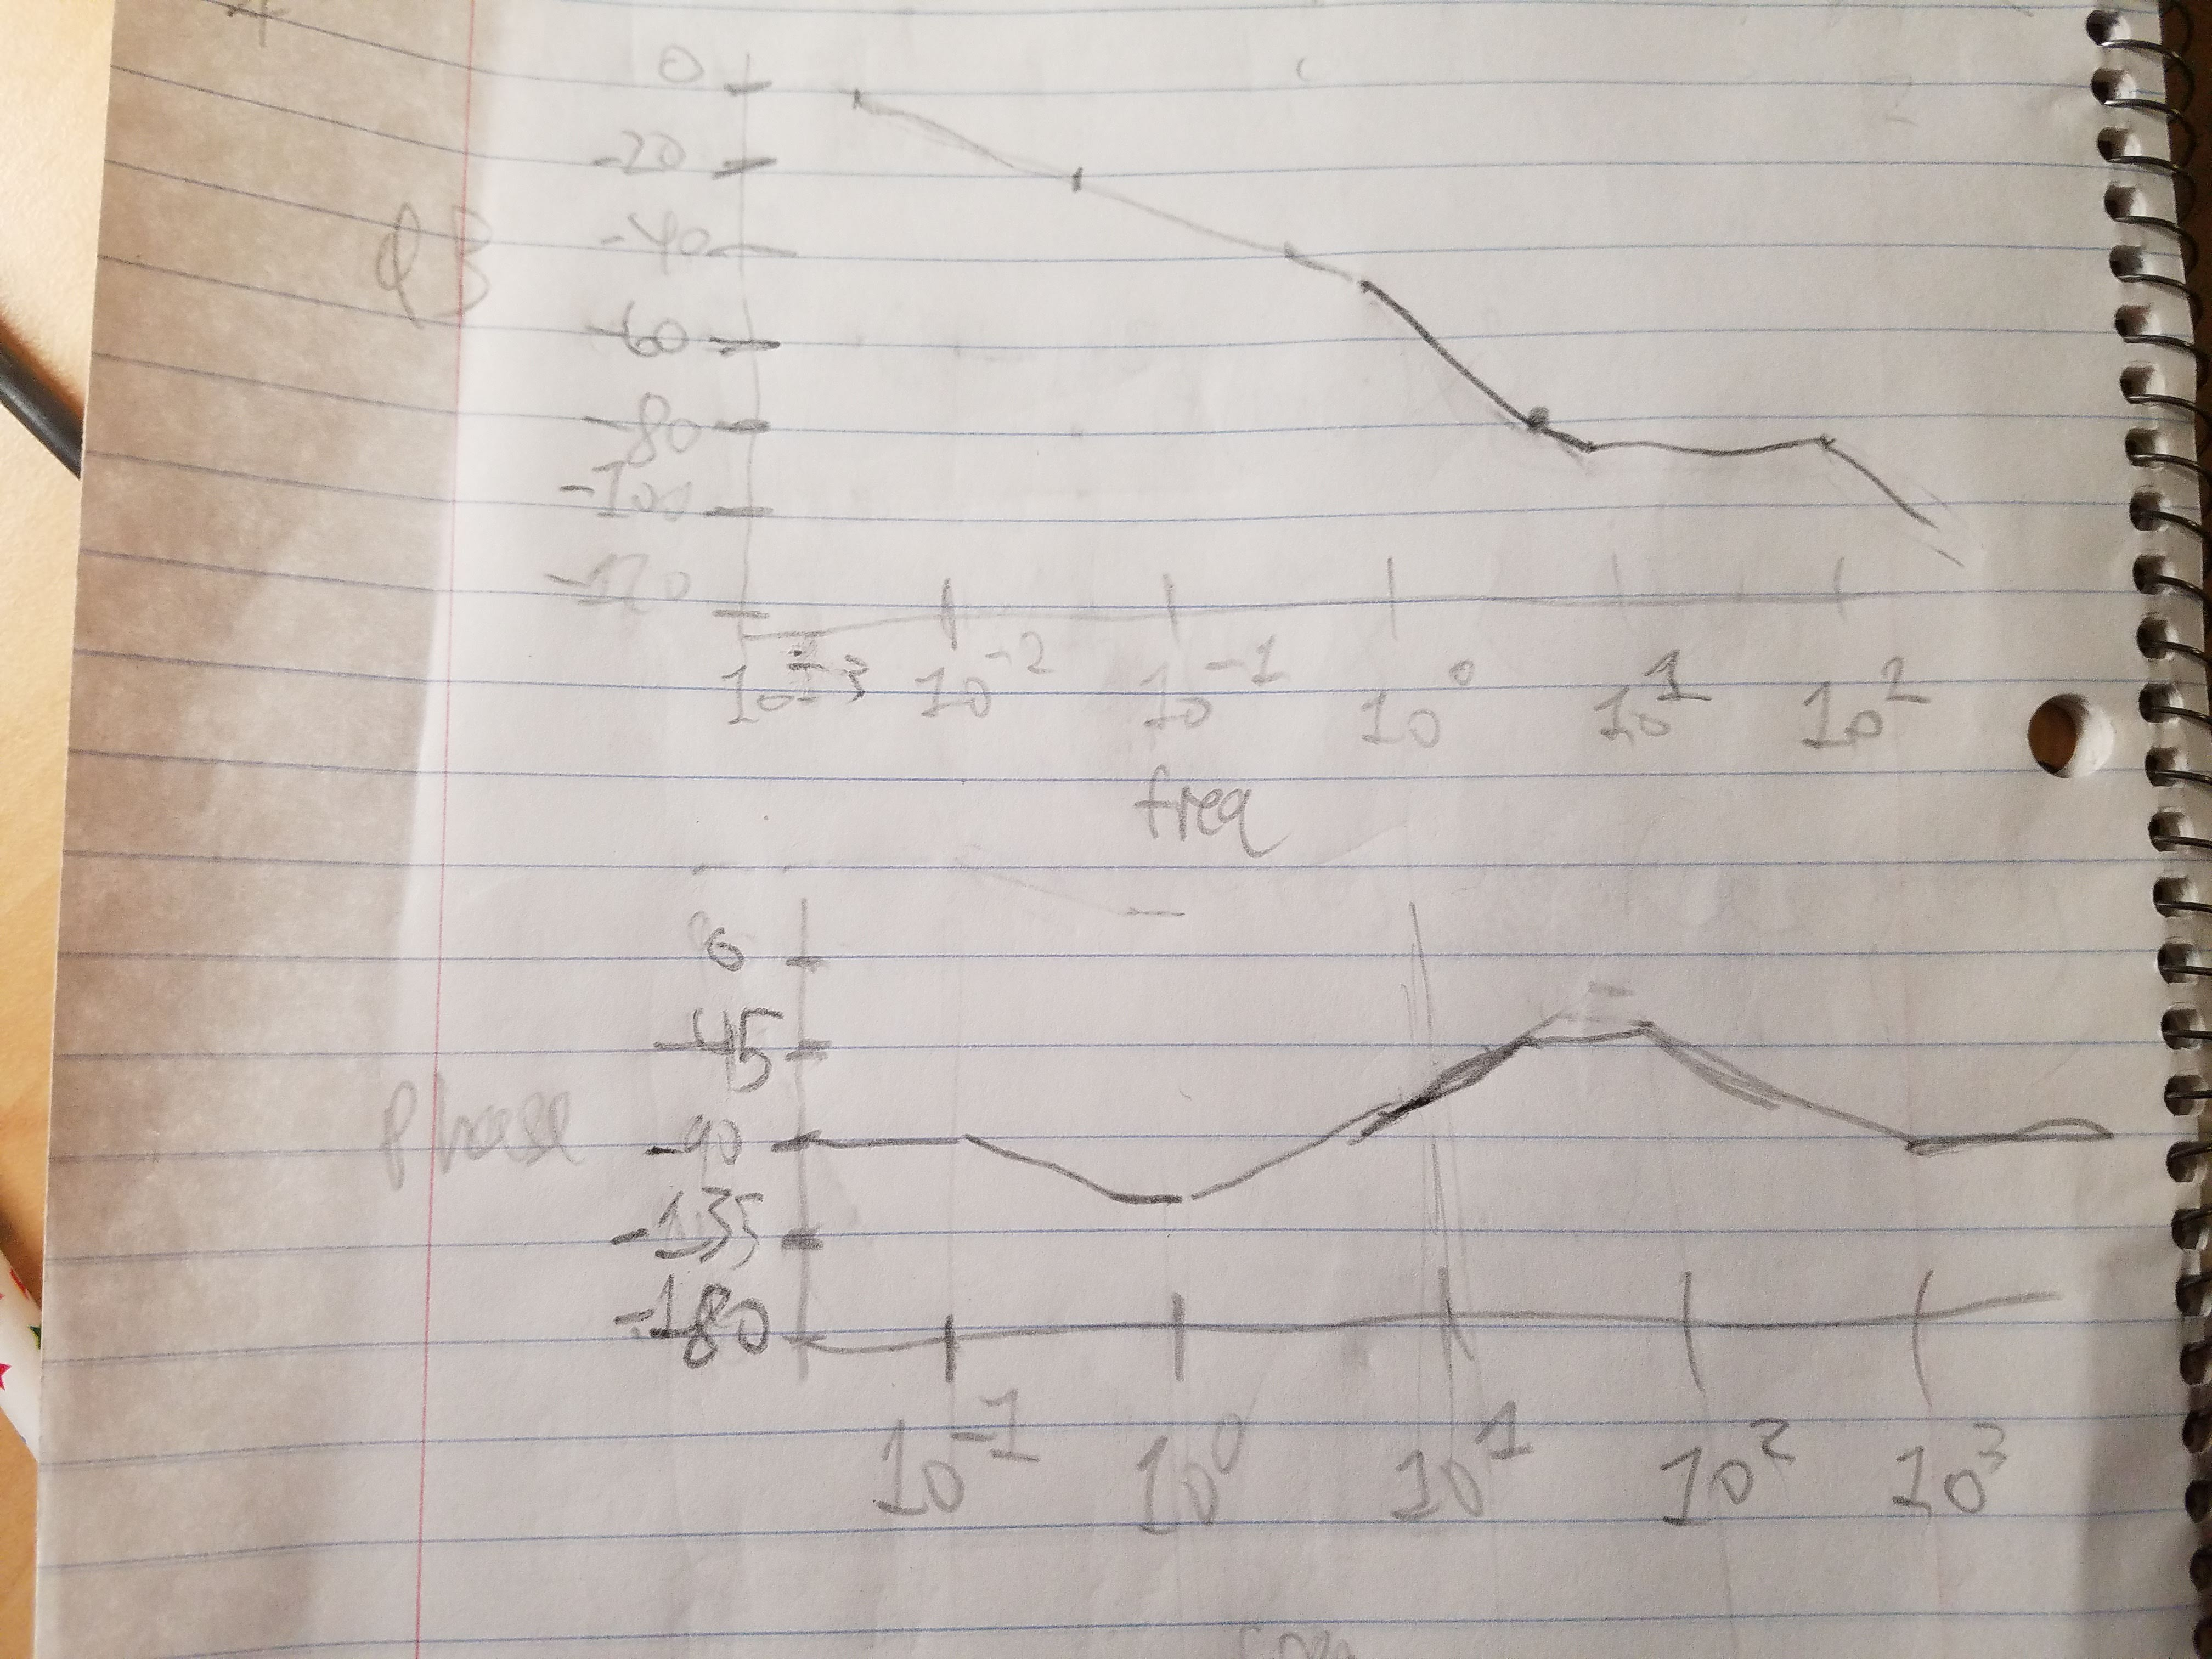
\includegraphics[width=2.5in]{problem1a.jpg}
        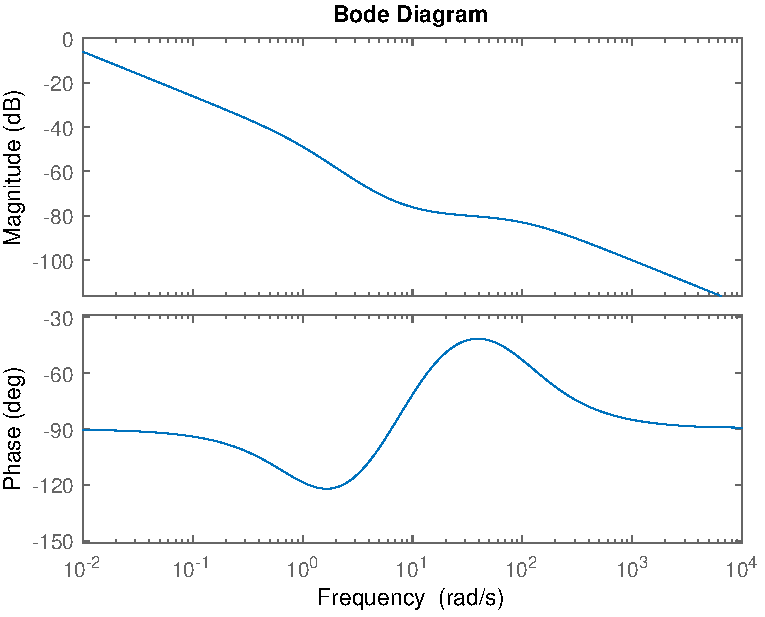
\includegraphics[width=2.5in]{problem1a.pdf}
    \end{center}
\end{figure}

\paragraph{b)}

This can be rewritten as follows.
\[L(s)=\frac{1}{s+1}\times\frac{1}{-s+1}\times s\]
The \(\frac{1}{-s+1}\) term produces the same magnitude as the first term but its phase goes to \(90\) instead of \(-90\) degrees since the imaginary component is reversed.
My asymptote sketch and the actual bode plot is shown below.
\begin{figure}[H]
    \begin{center}
        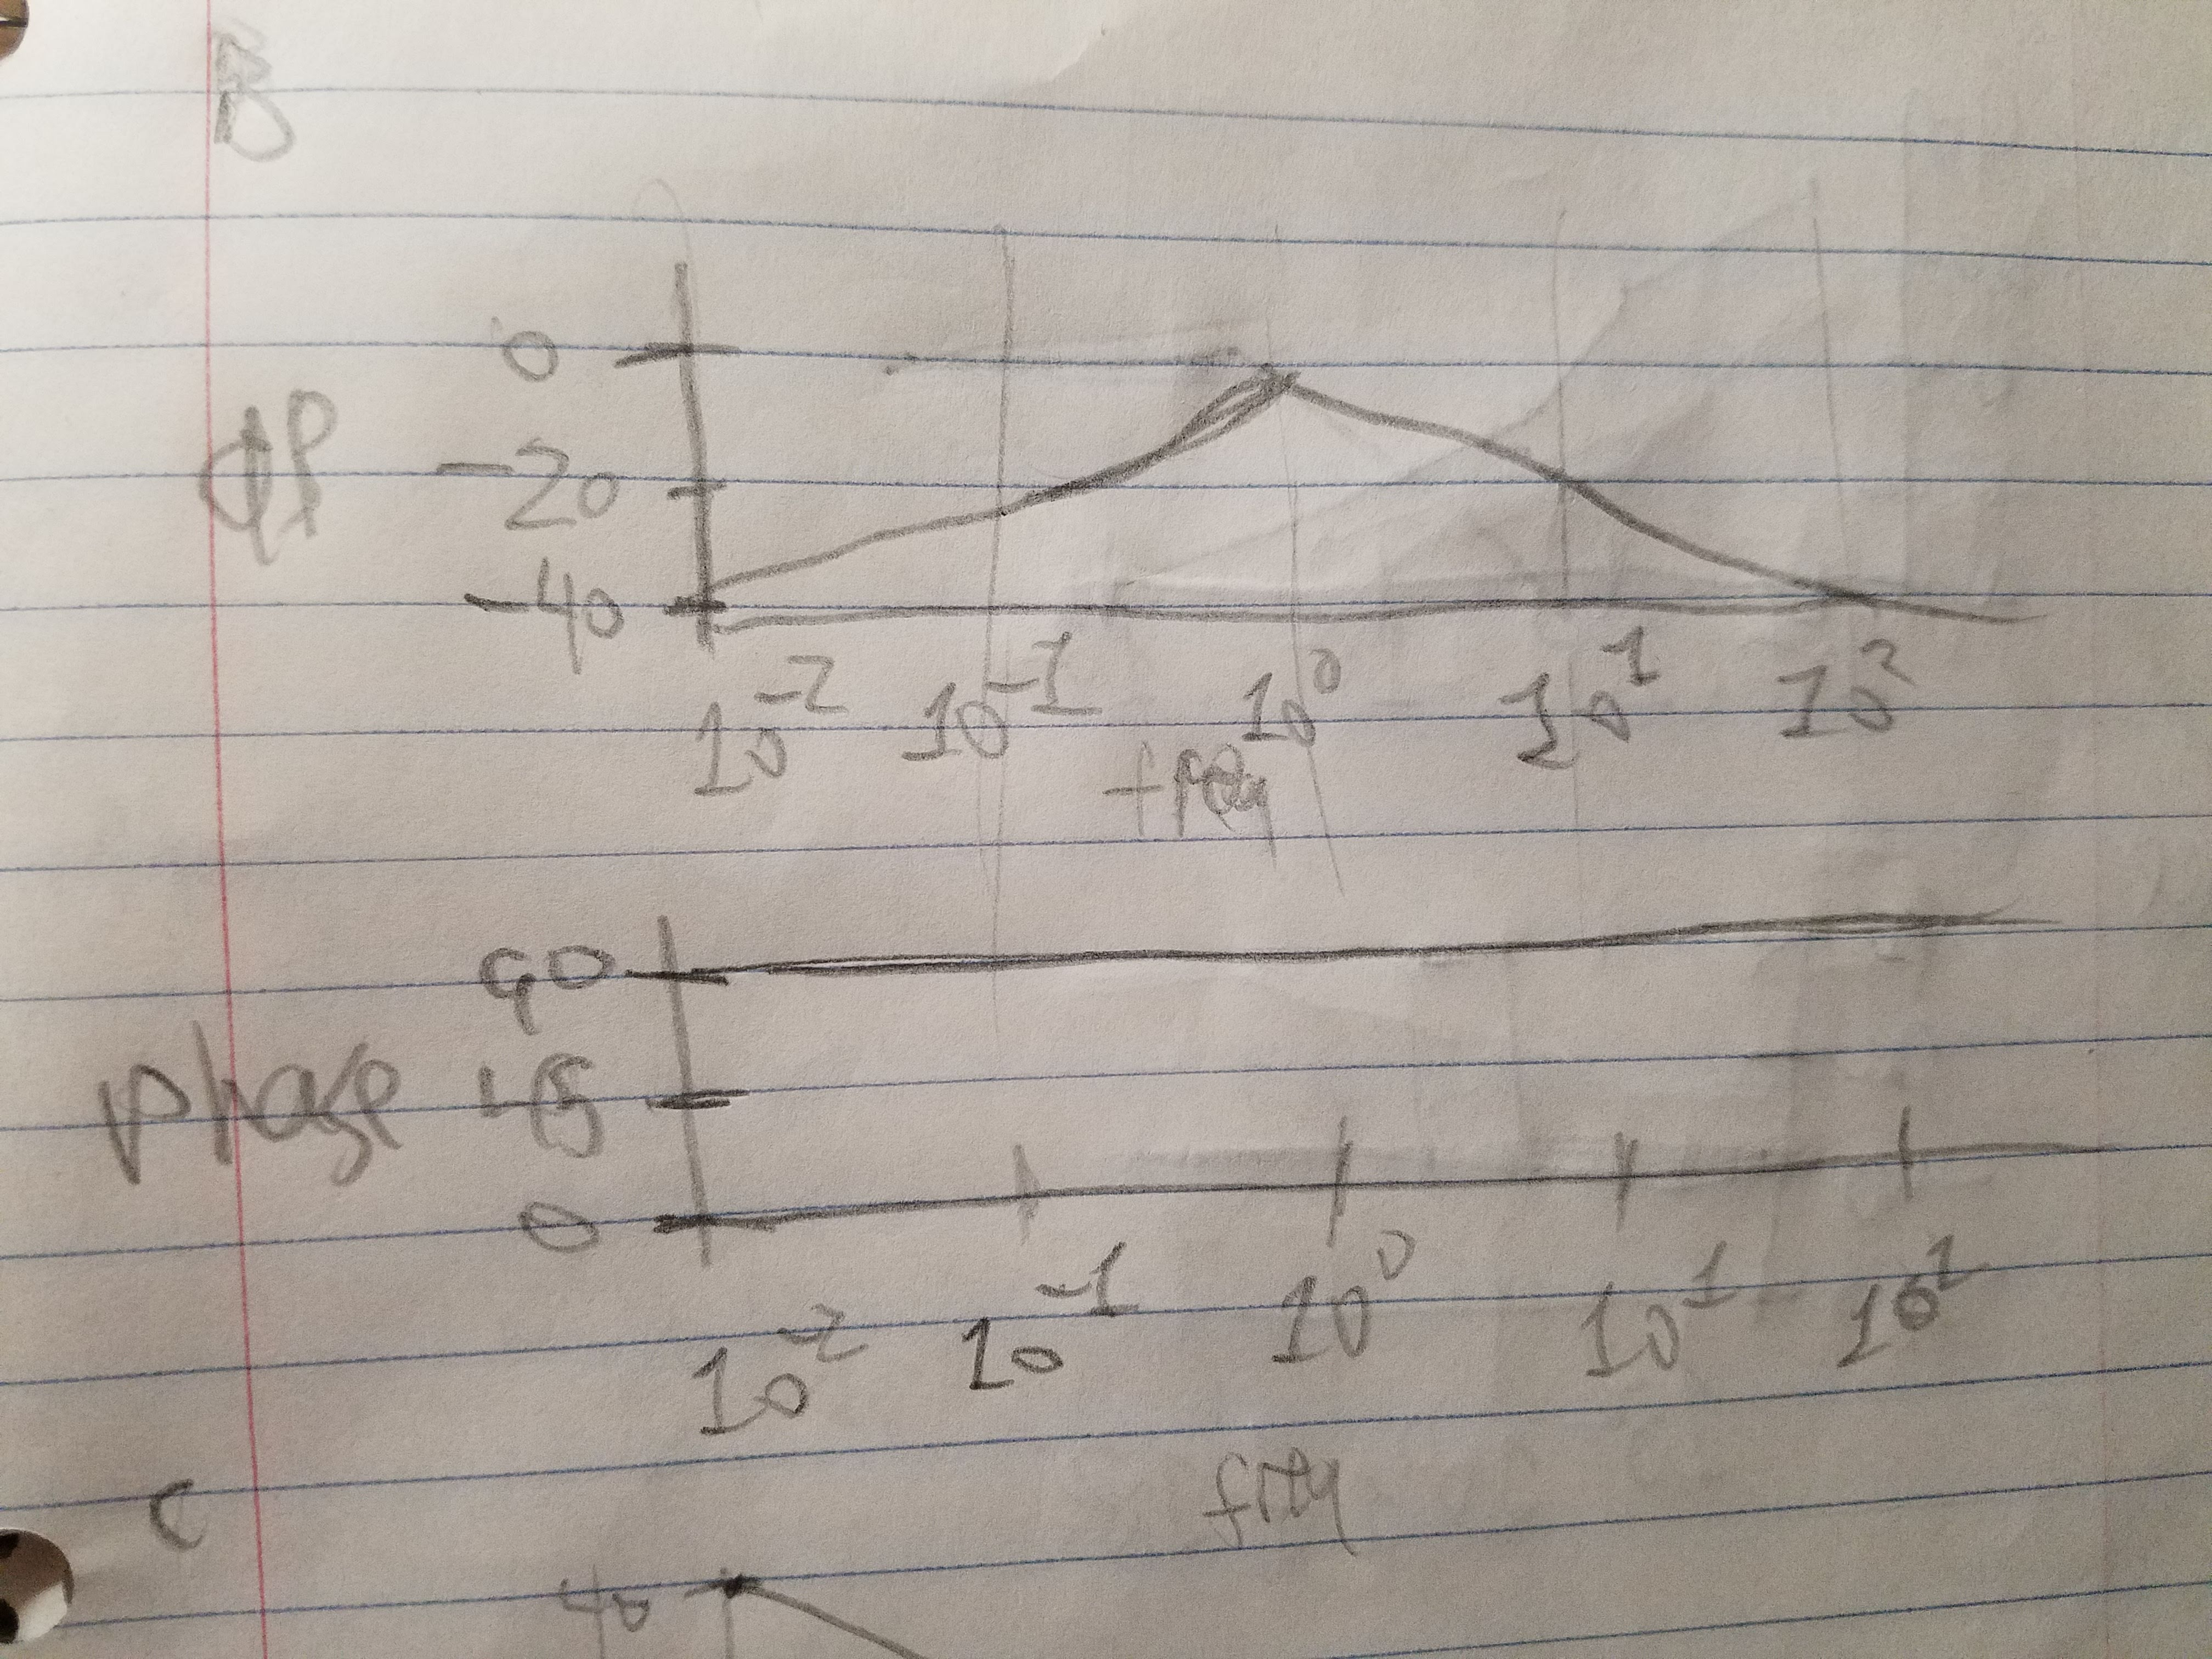
\includegraphics[width=2.5in]{problem1b.jpg}
        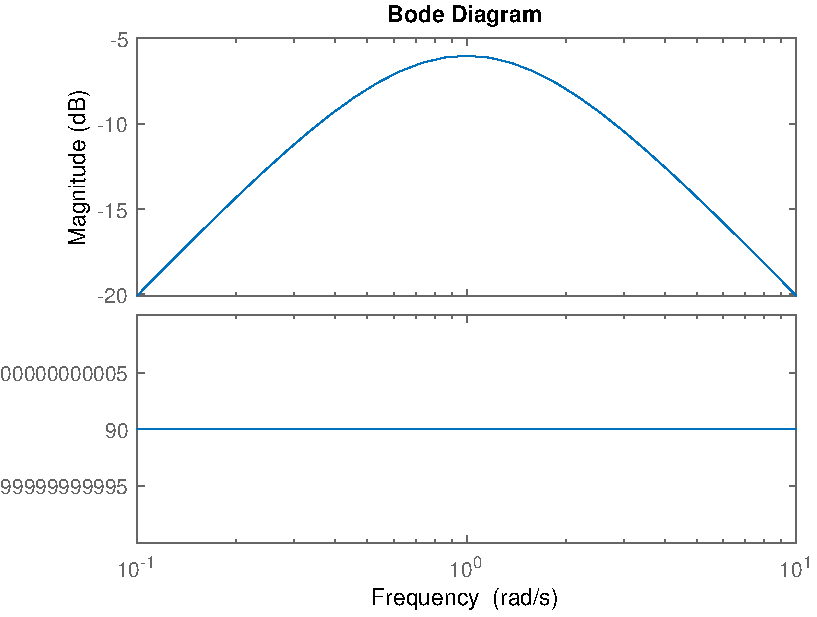
\includegraphics[width=2.5in]{problem1b.pdf}
    \end{center}
\end{figure}

\paragraph{c)}

This can be rewritten as follows.
\[L(s)=\frac{1}{s}\times\frac{1}{s+1}\times(-s+1)\]
The \(-s+1\) term has a phase that goes from 0 degrees to \(-90\) degrees since the imaginary component is reversed.
My asymptote sketch and the actual bode plot is shown below.
\begin{figure}[H]
    \begin{center}
        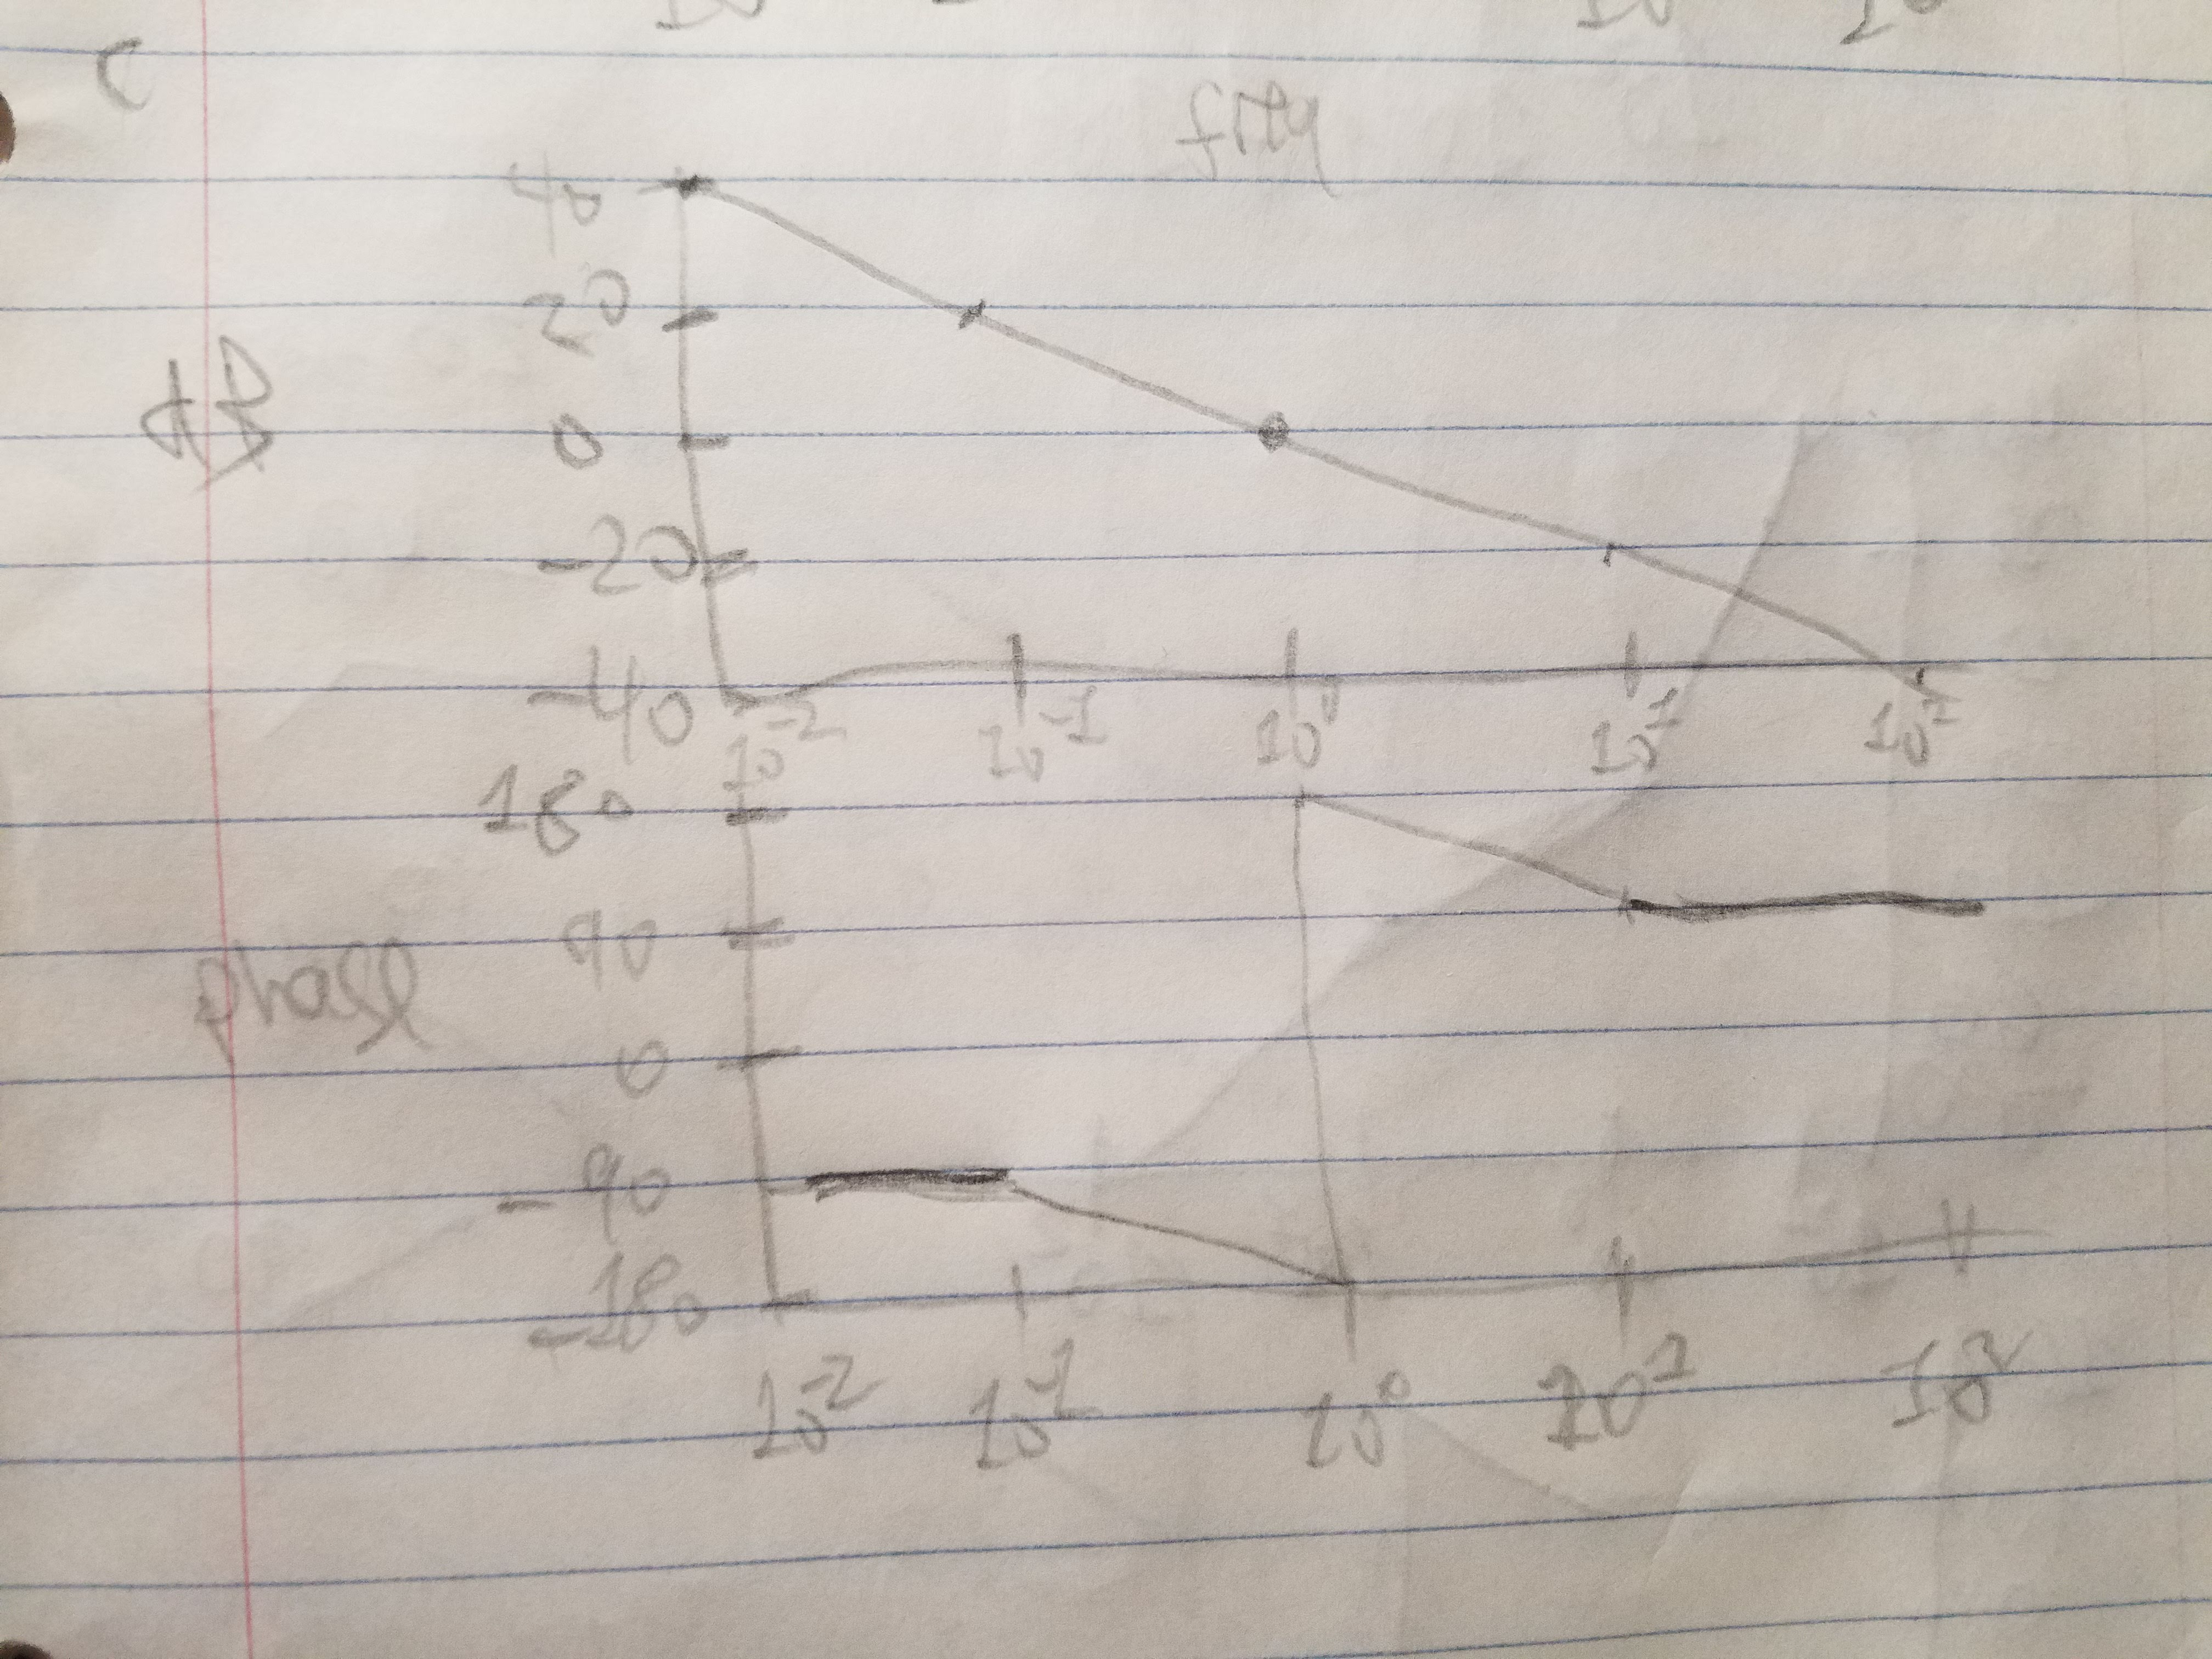
\includegraphics[width=2.5in]{problem1c.jpg}
        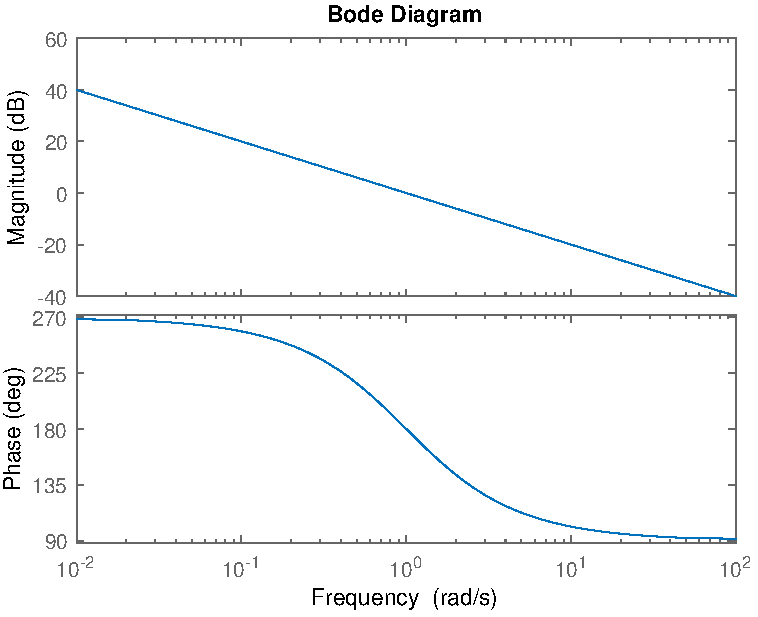
\includegraphics[width=2.5in]{problem1c.pdf}
    \end{center}
\end{figure}

\paragraph{d)}

This can be rewritten as follows.
\[L(s)=4\times\frac{1}{s}\times\frac{1}{s^2+1}\times\left(\left(\frac{s}{2}\right)^2+1\right)\]
The \(\frac{1}{s^2+1}\) term will have a phase that jumps immediately from 0 to \(-180\) after \(\omega=1\). Similarly
the quadratic term in the numerator will have a phase that jumps from 0 to \(180\) after \(\omega=2\). It has a magnitude asymptote
that increases at 40 decibels every decade after this point as well.
My asymptote sketch and the actual bode plot is shown below.
\begin{figure}[H]
    \begin{center}
        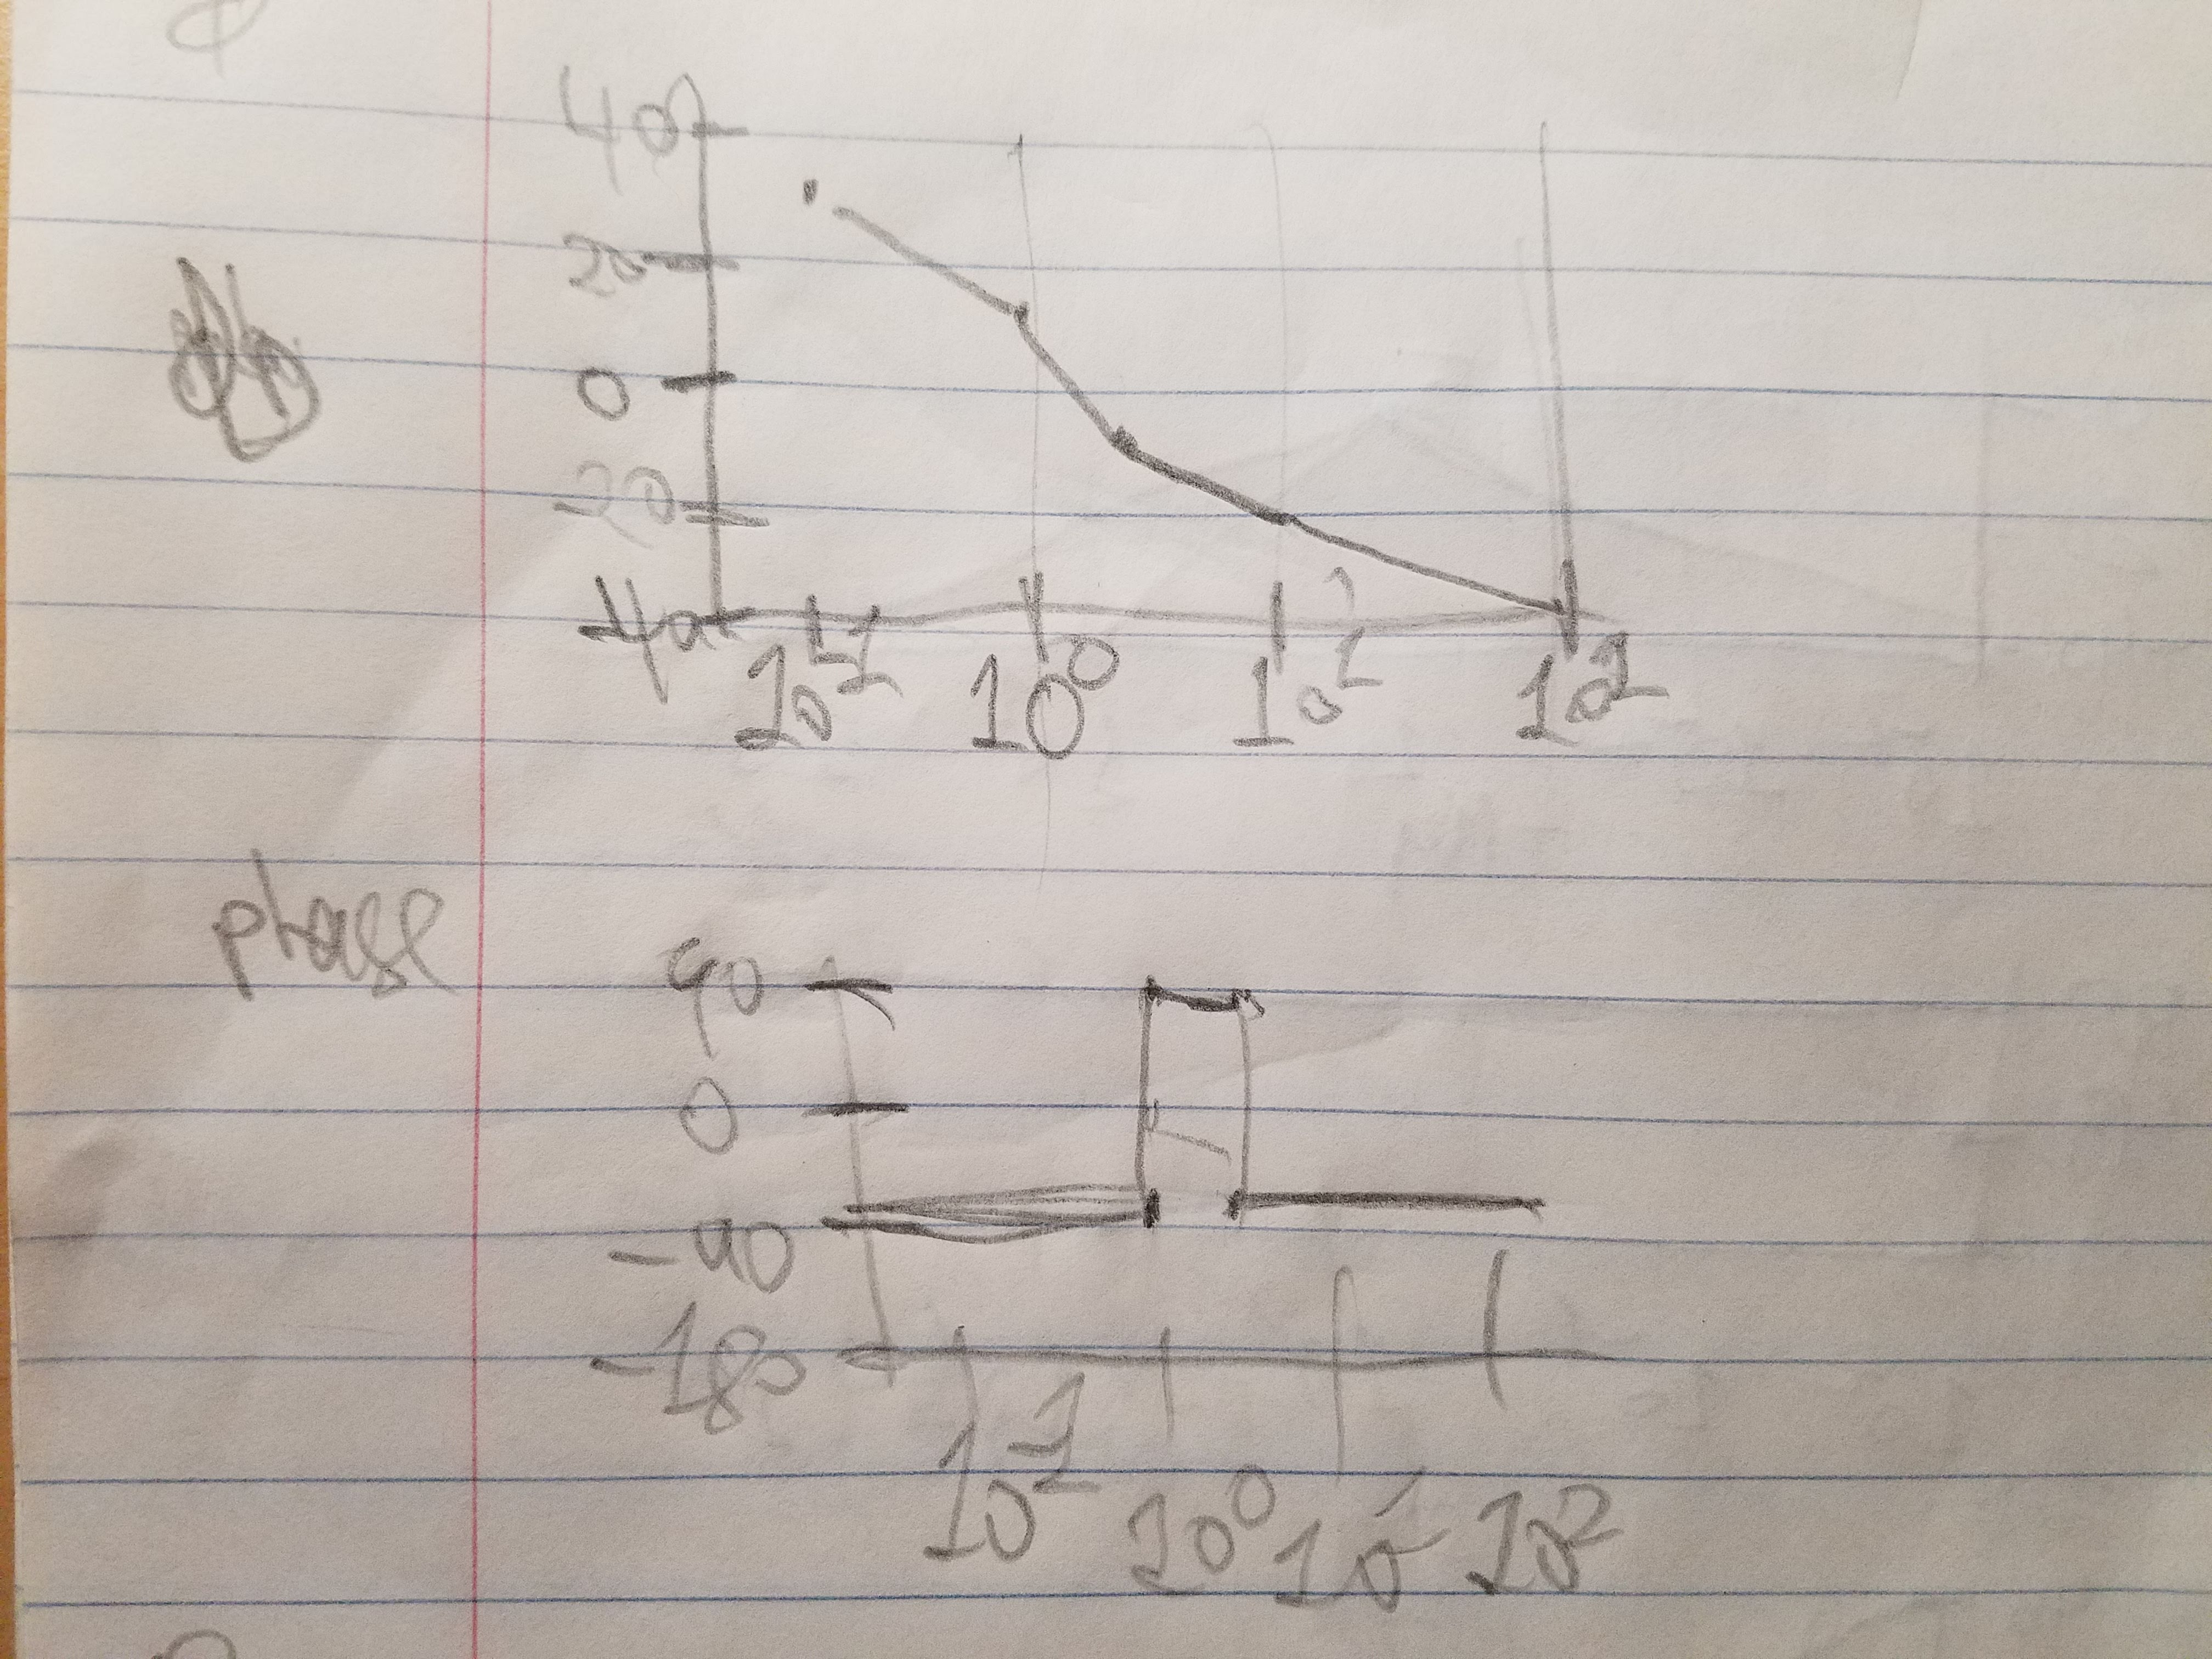
\includegraphics[width=2.5in]{problem1d.jpg}
        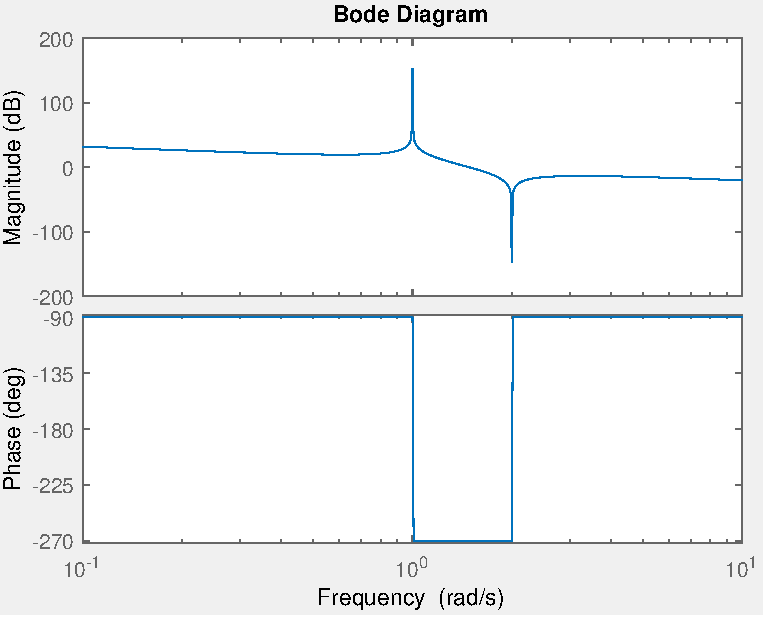
\includegraphics[width=2.5in]{problem1d.pdf}
    \end{center}
\end{figure}

\paragraph{e)}

This can be rewritten as follows.
\[L(s)=\frac{1}{10}\times\frac{1}{s^3}\times\frac{1}{\frac{1}{10}s+1}\times(s+1)\times(s+1)\]
My asymptote sketch and the actual bode plot is shown below.
\begin{figure}[H]
    \begin{center}
        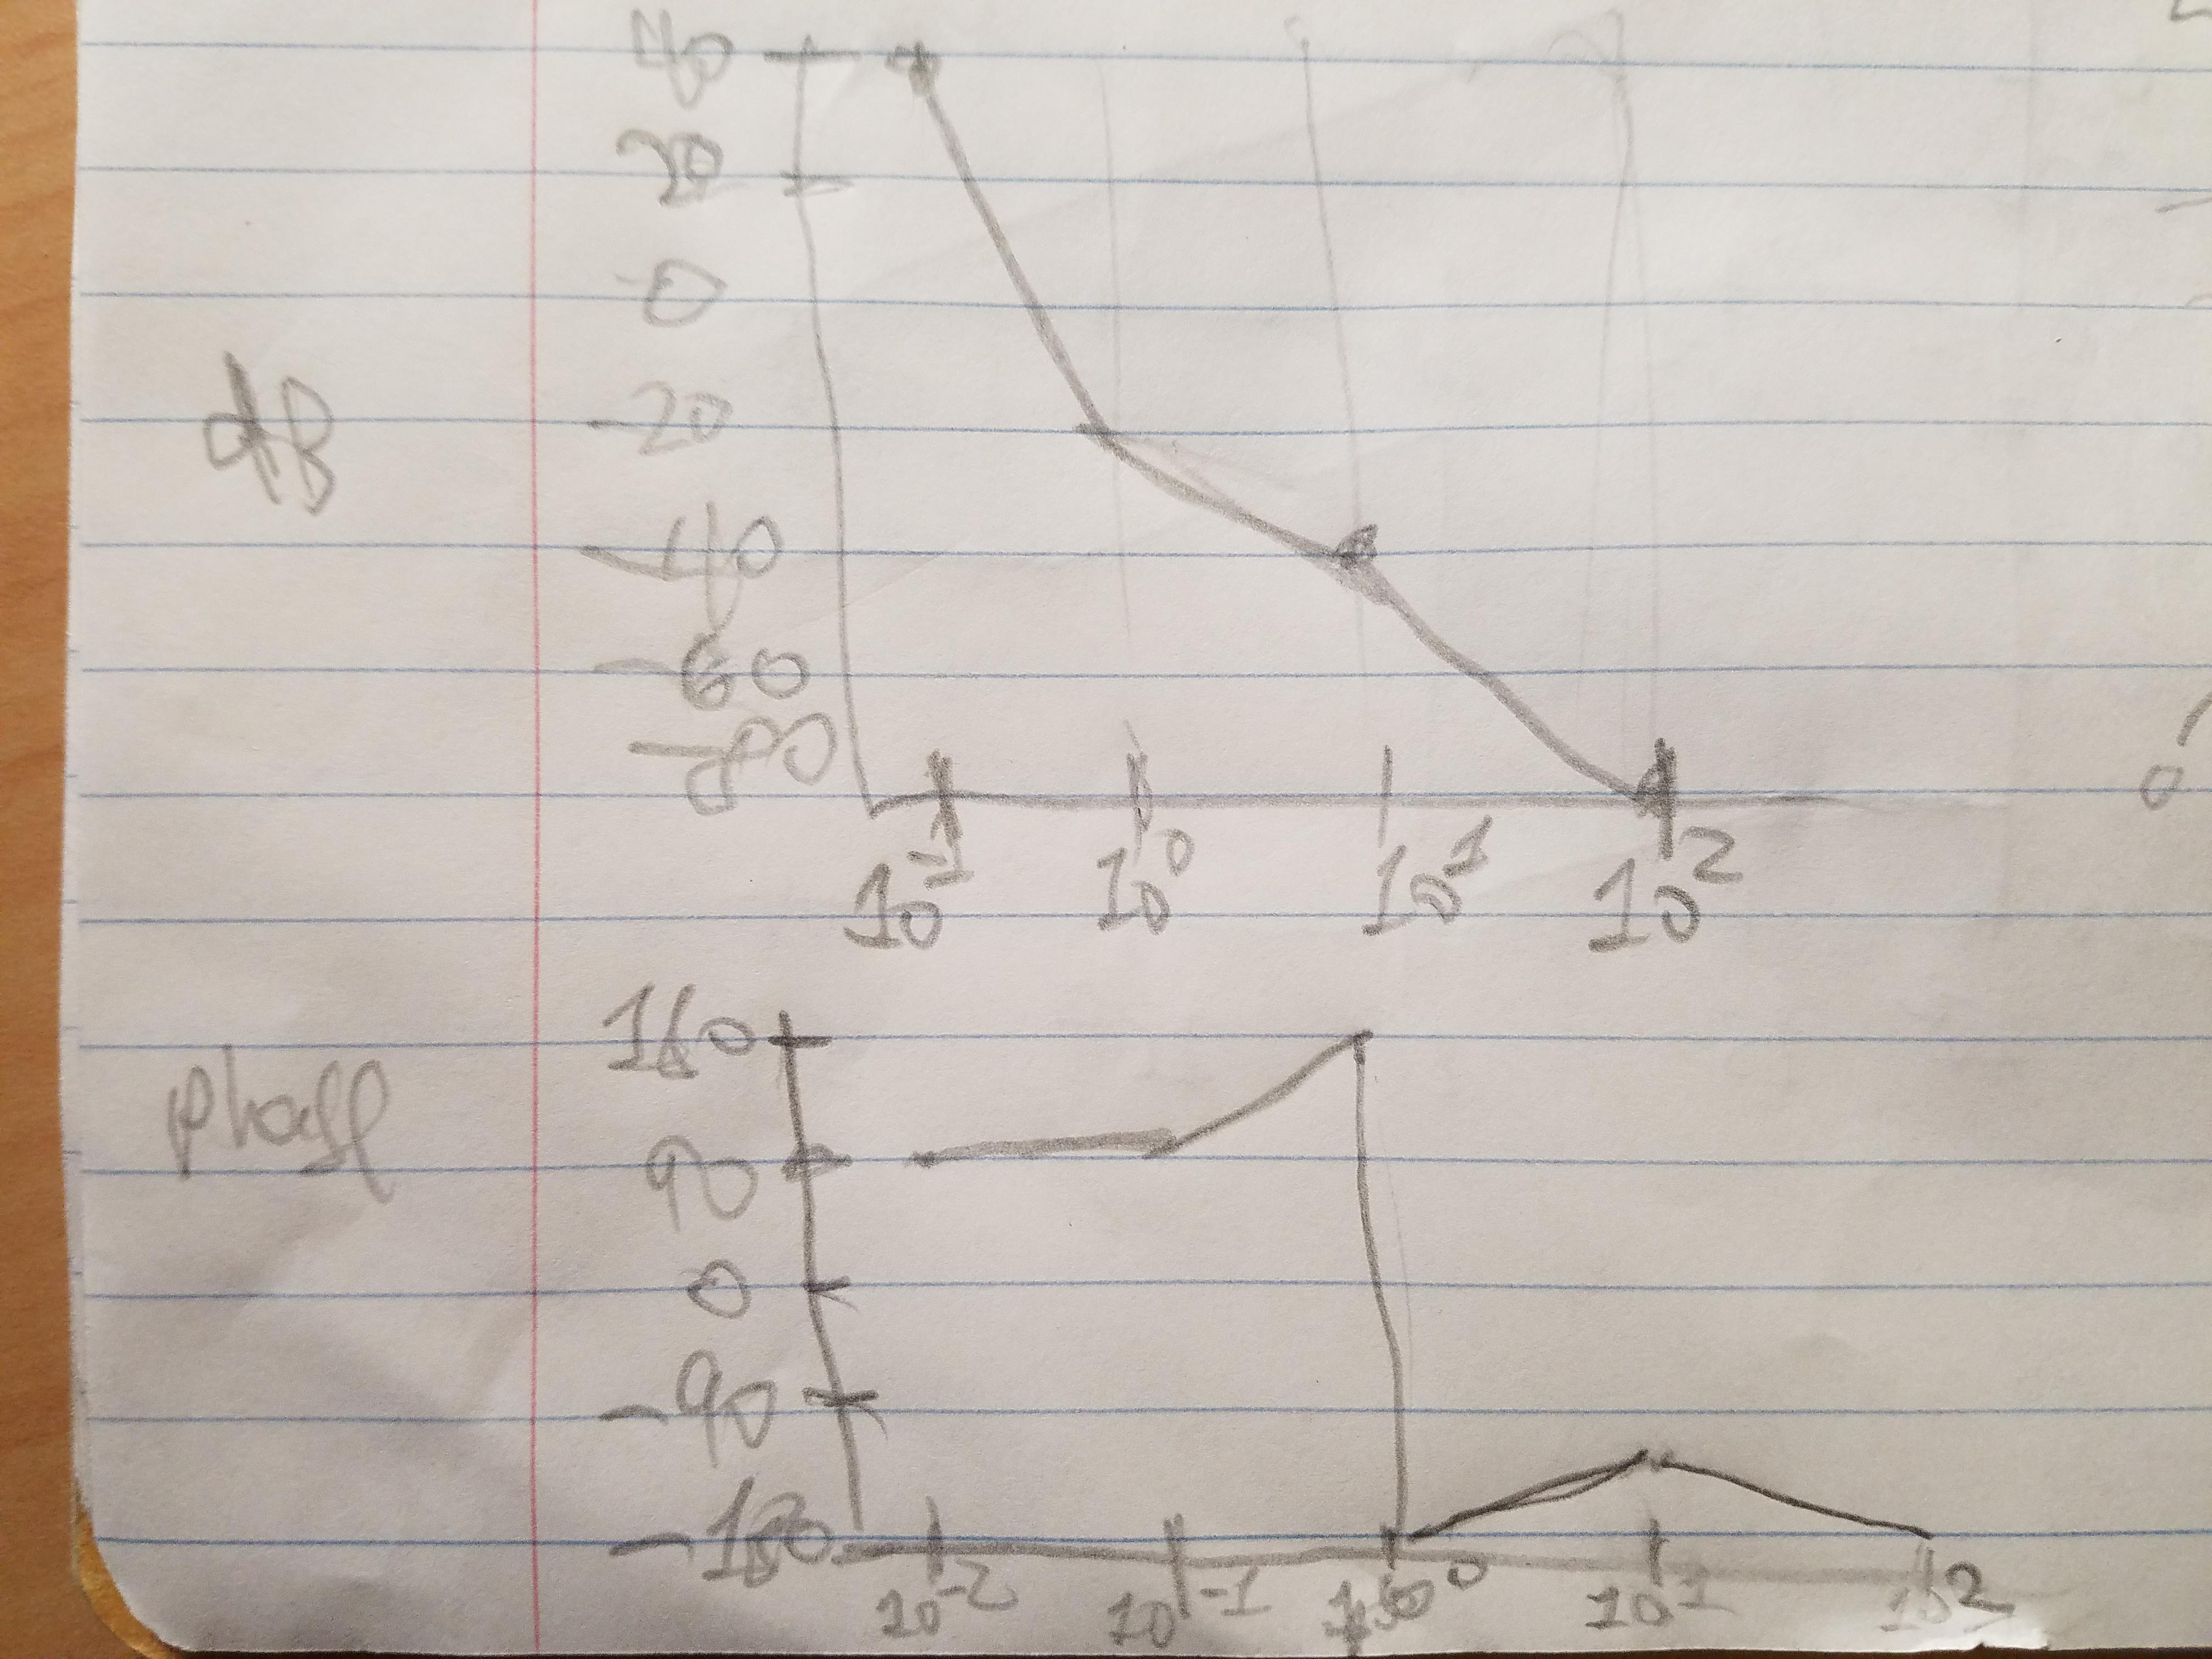
\includegraphics[width=2.5in]{problem1e.jpg}
        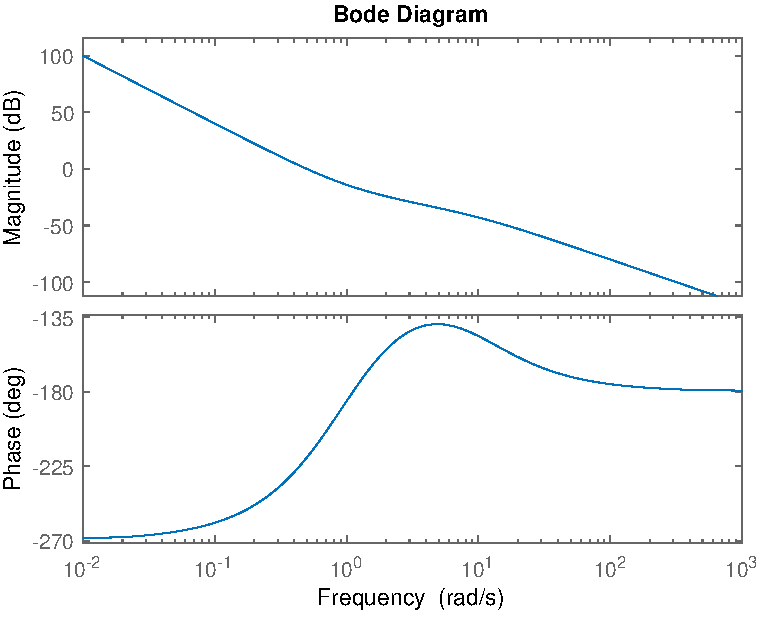
\includegraphics[width=2.5in]{problem1e.pdf}
    \end{center}
\end{figure}

\paragraph{f)}

This can be rewritten as follows.
\[L(s)=e^{-0.2s}\times\frac{1}{s}\times\frac{1}{s+1}\]
The exponential term has no effect on the magnitude. It will cause the phase to rapidly move cycle through all the angles as the frequency
increases, so there is no use predicting the asymptote for frequencies greater than 1.
My asymptote sketch and the actual bode plot is shown below.
\begin{figure}[H]
    \begin{center}
        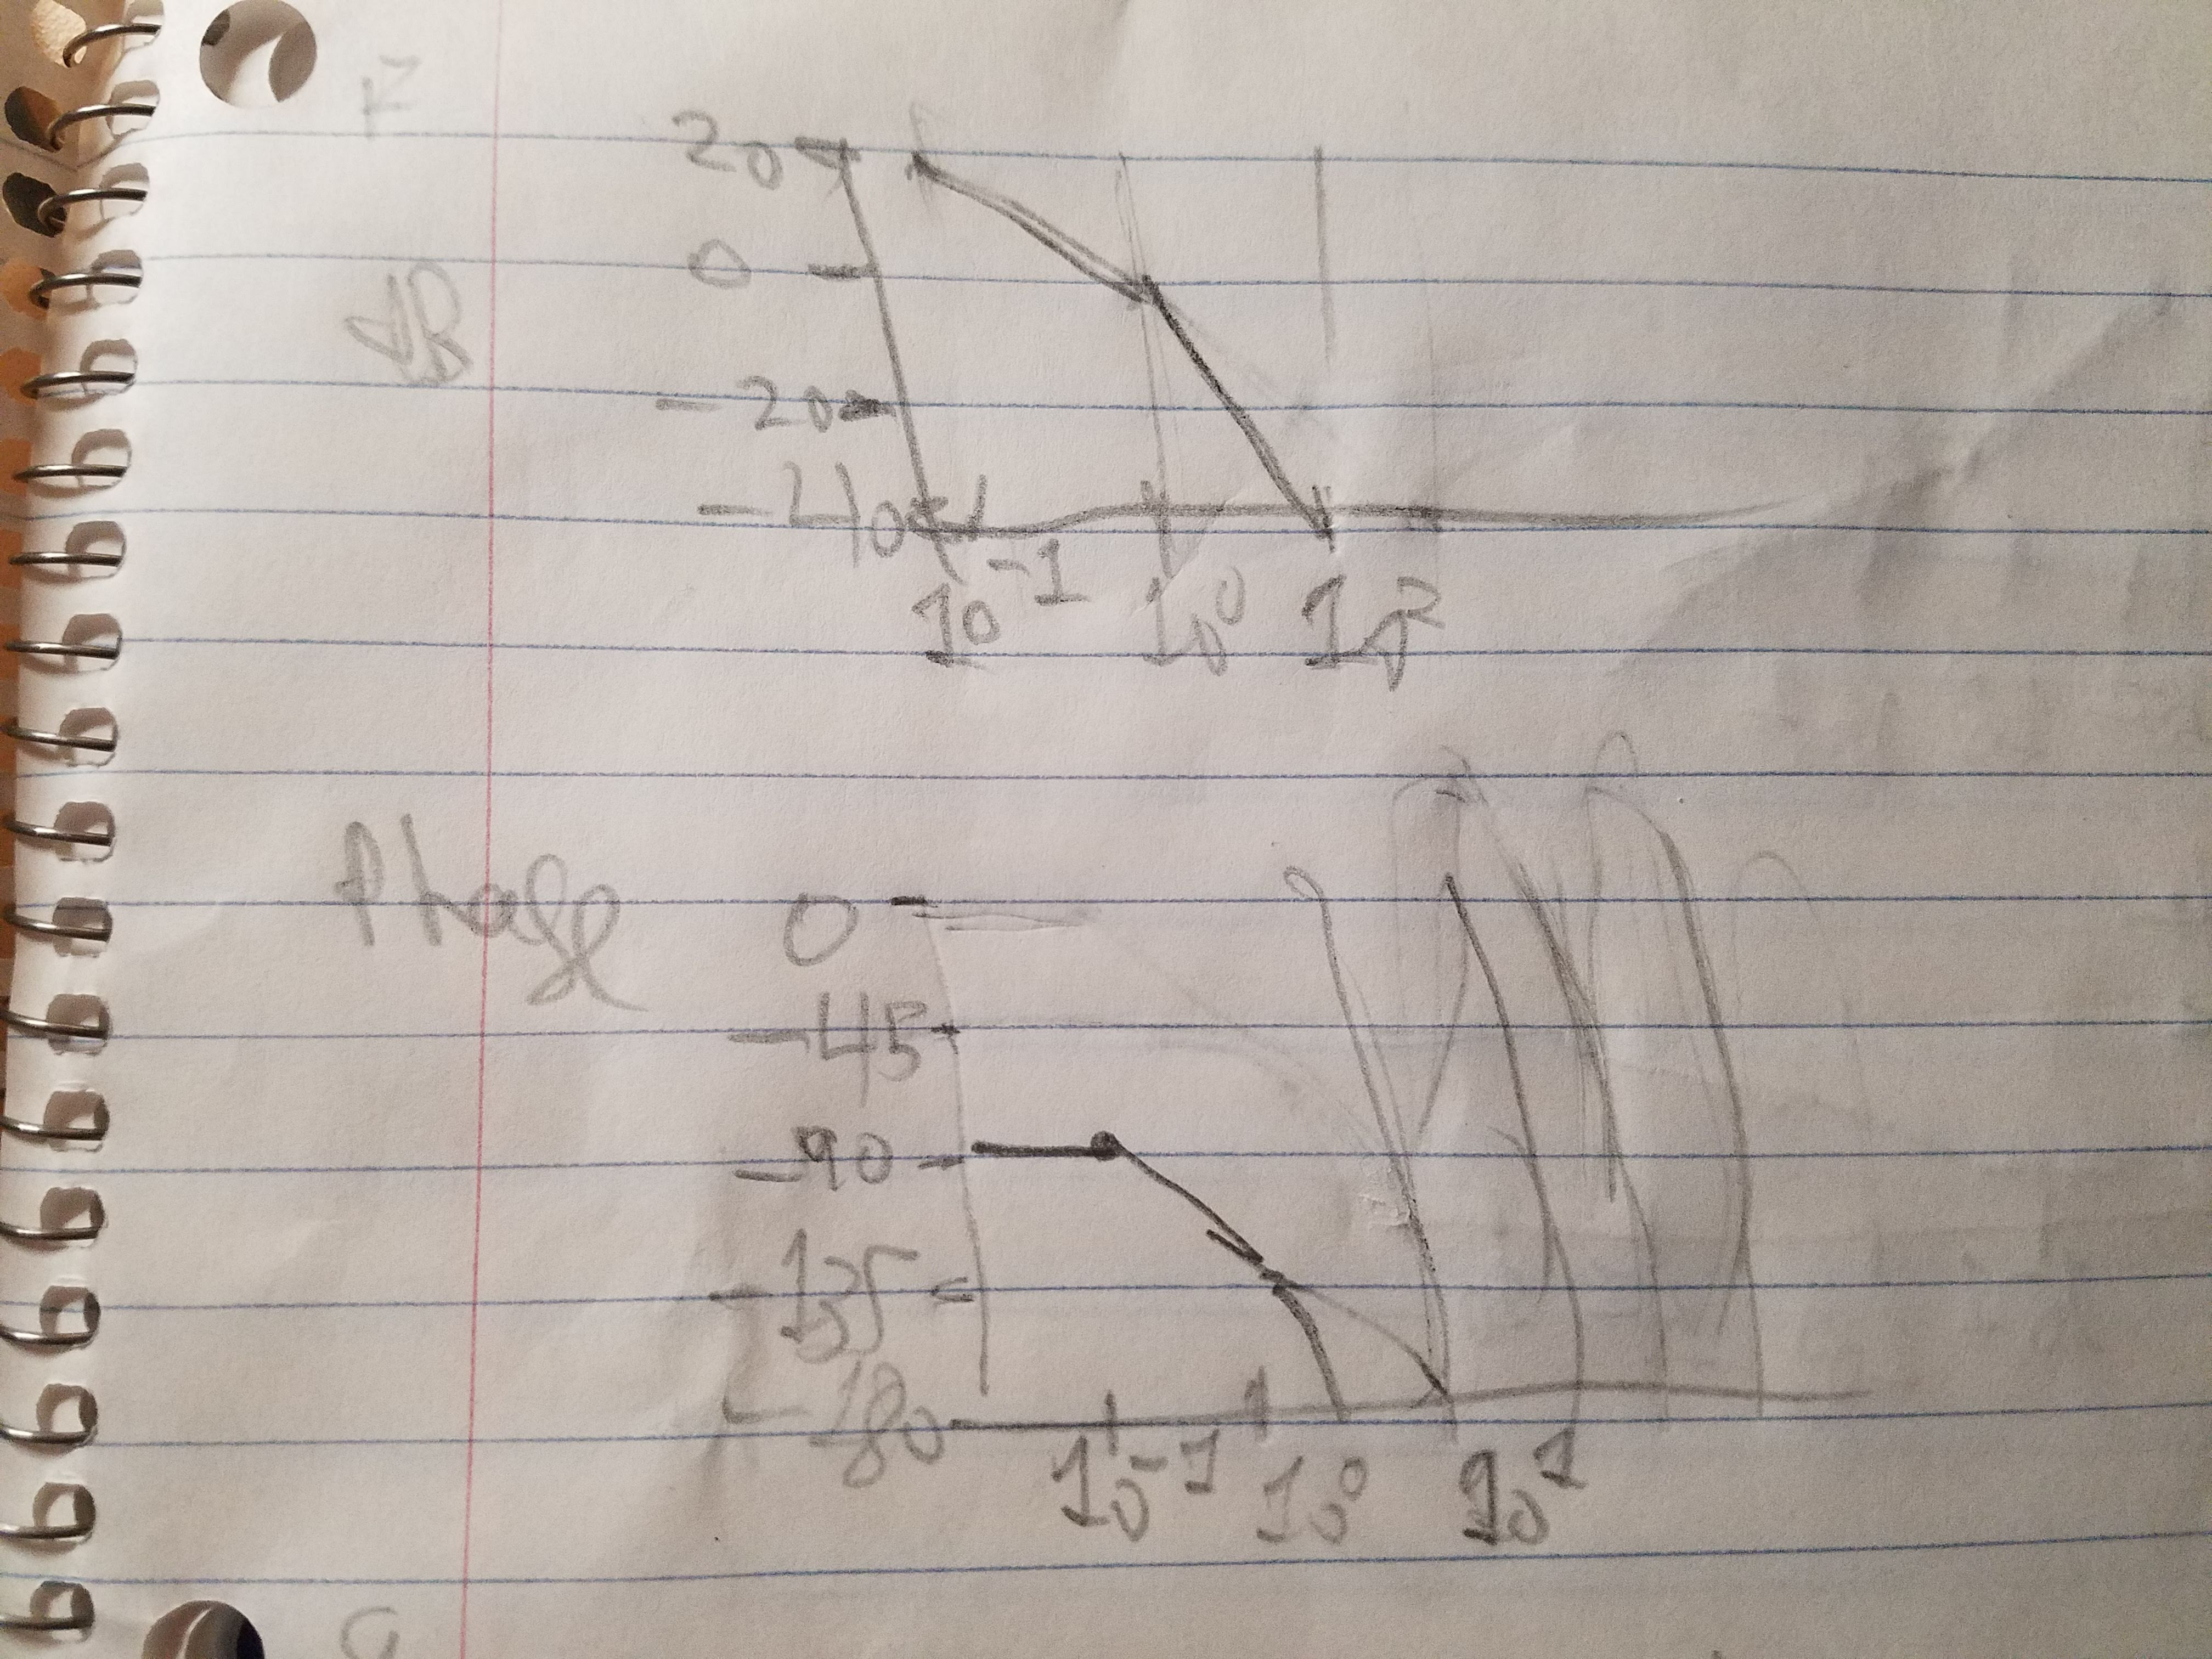
\includegraphics[width=2.5in]{problem1f.jpg}
        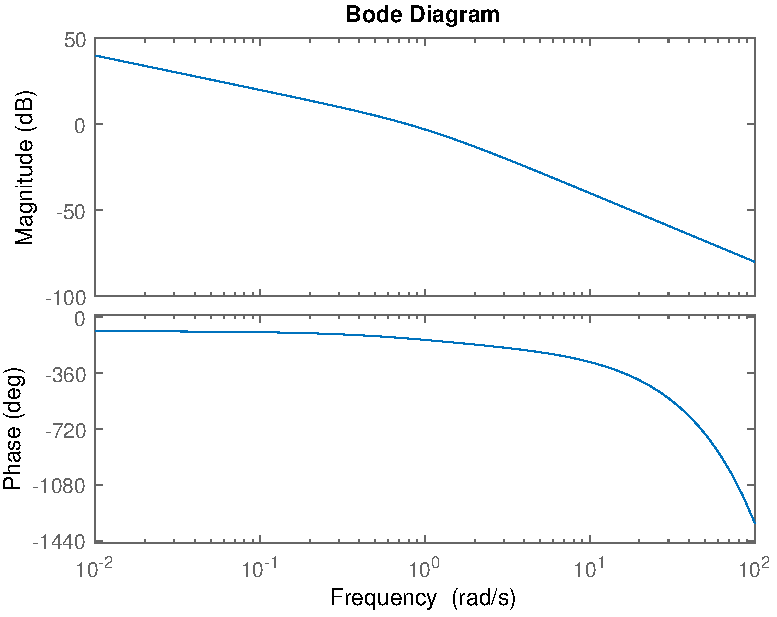
\includegraphics[width=2.5in]{problem1f.pdf}
    \end{center}
\end{figure}

\paragraph{g)}

This can be rewritten as follows.
\[L(s)=\frac{1}{10}\times\frac{1}{s}\times\frac{100}{s^2+20s+100}\times(s+1)\]
My asymptote sketch and the actual bode plot is shown below.
\begin{figure}[H]
    \begin{center}
        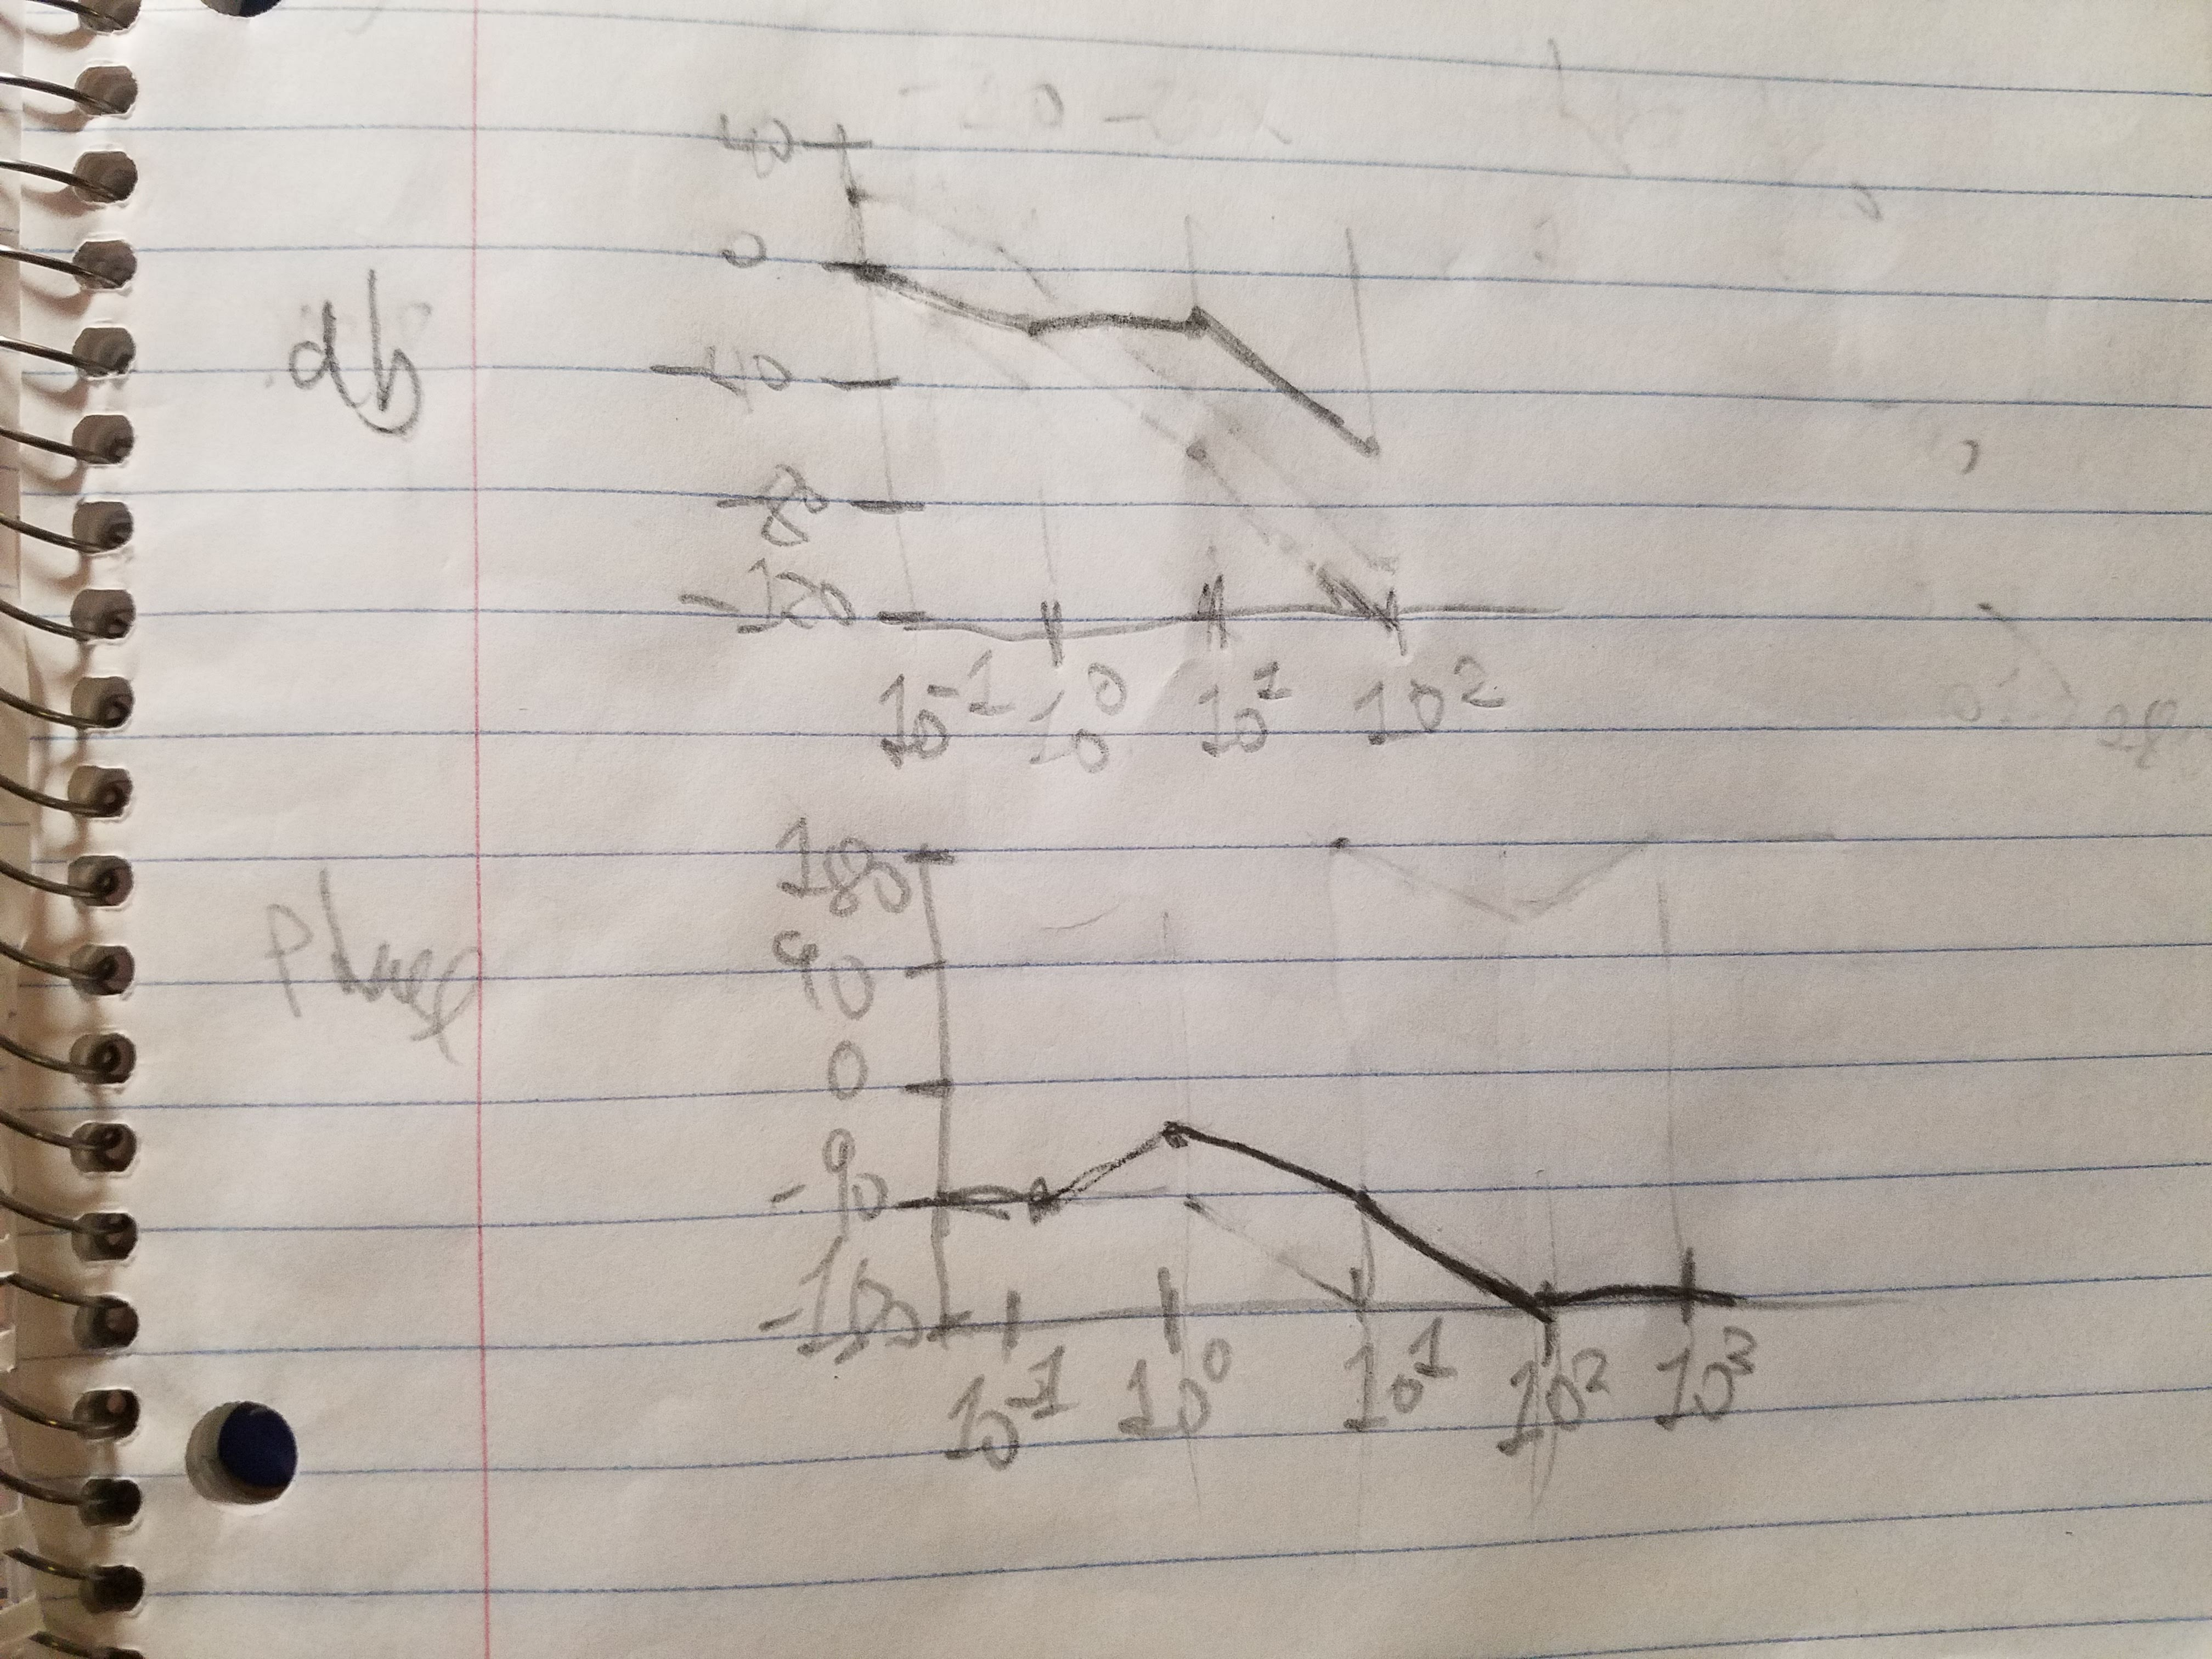
\includegraphics[width=2.5in]{problem1g.jpg}
        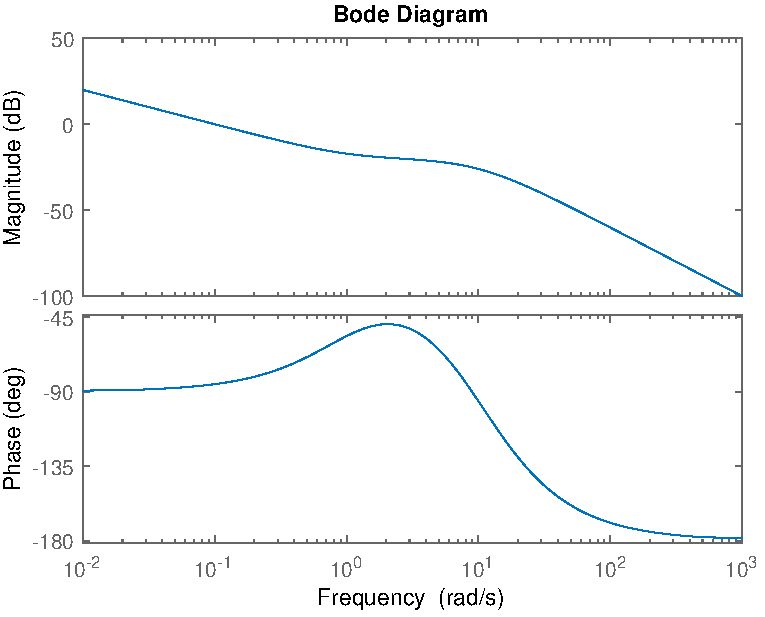
\includegraphics[width=2.5in]{problem1g.pdf}
    \end{center}
\end{figure}

\paragraph{h)}
This can be rewritten as follows.
\[L(s)=\frac{1}{s^2}\times\left(\frac{1}{2}s+1\right)\]
My asymptote sketch and the actual bode plot is shown below.
\begin{figure}[H]
    \begin{center}
        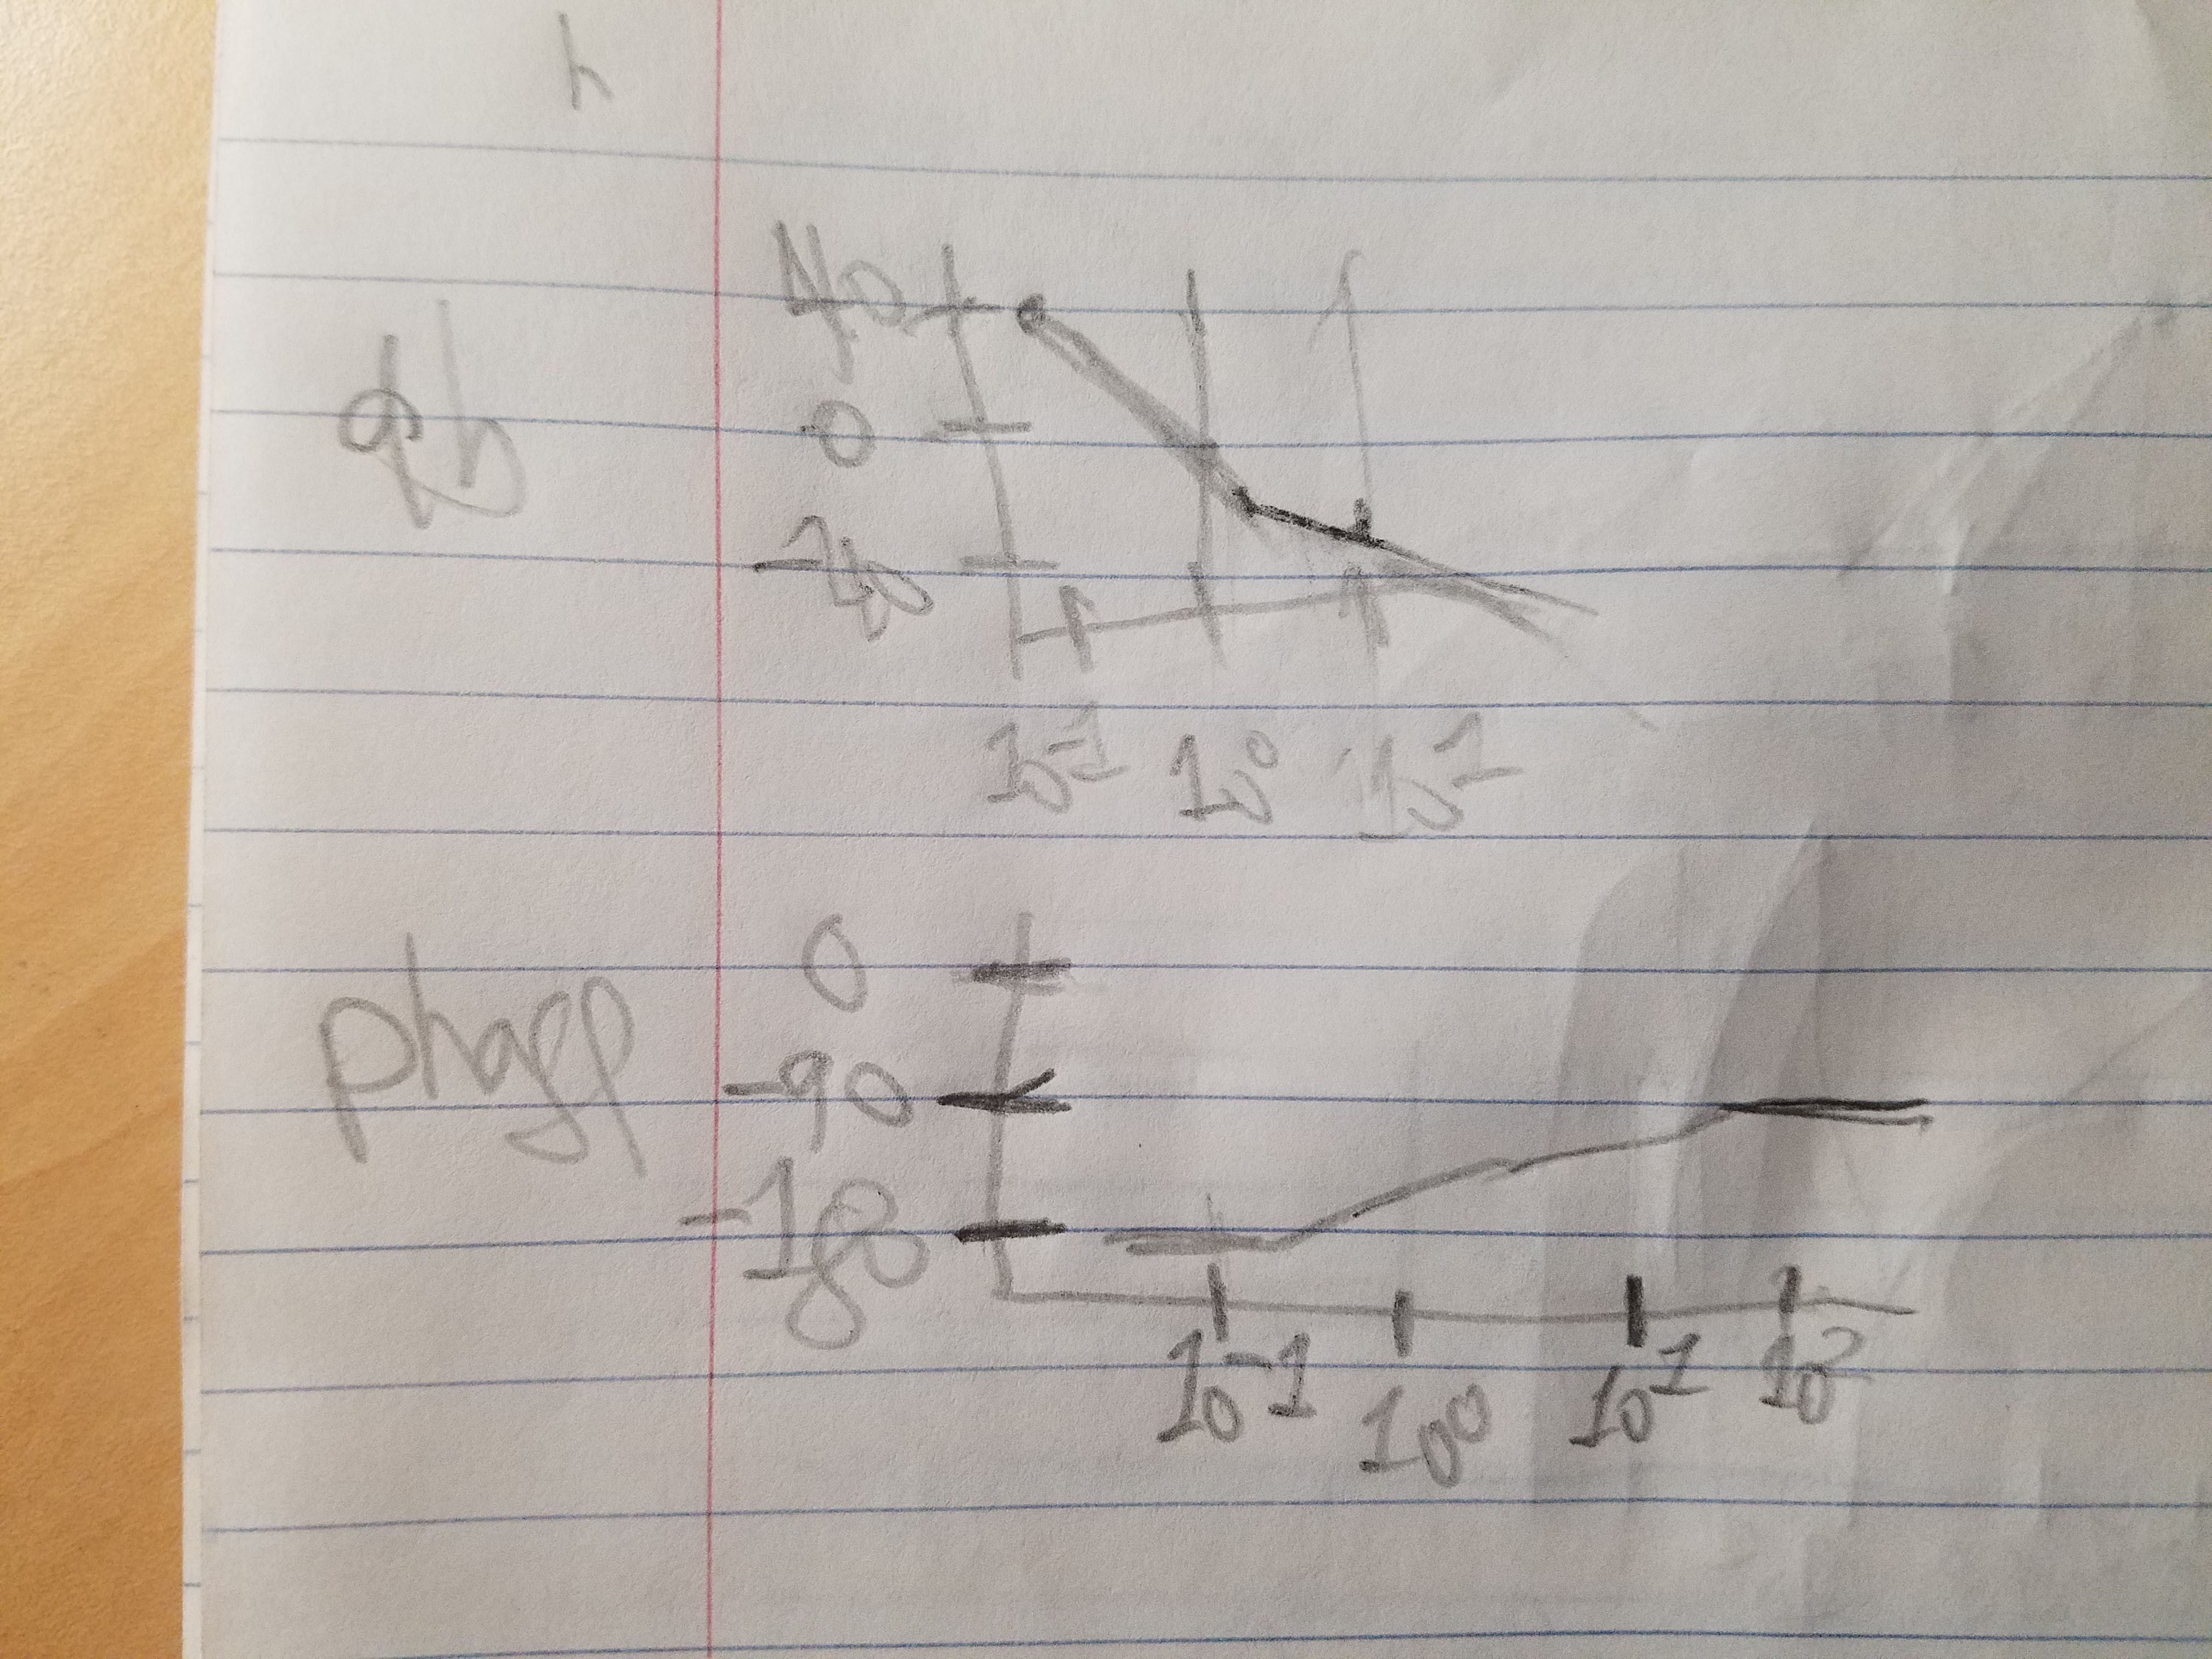
\includegraphics[width=2.5in]{problem1h.jpg}
        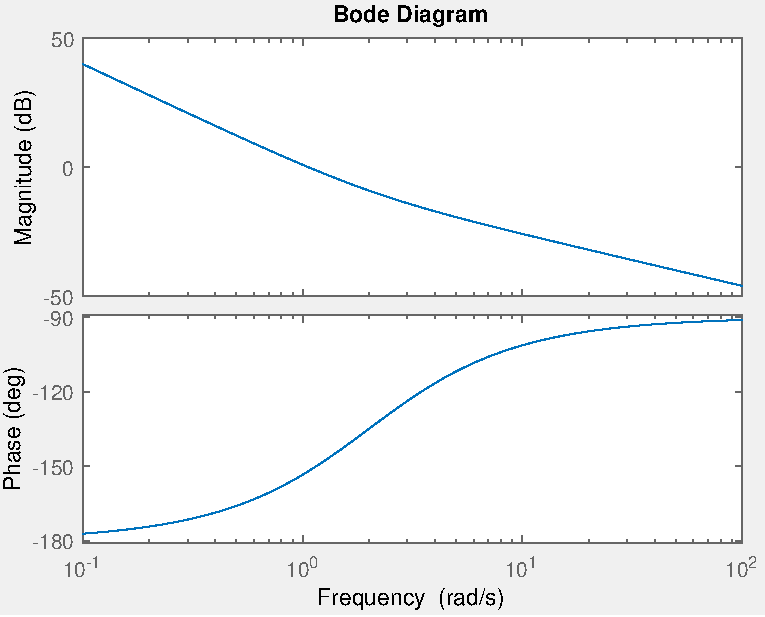
\includegraphics[width=2.5in]{problem1h.pdf}
    \end{center}
\end{figure}

\section*{Problem 2}

\paragraph{a)}

I ran the following code.
\begin{verbatim}
s=tf('s');
H1=(s/0.01+1)/(s^2+s+1);
H2=(s/0.1+1)/(s^2+s+1);
H3=(s/1+1)/(s^2+s+1);
H4=(s/10+1)/(s^2+s+1);
H5=(s/100+1)/(s^2+s+1);

set(gcf,'color','w');
step(H1);
hold on;
step(H2);
step(H3);
step(H4);
step(H5);
hold off;
export_fig problem2a.pdf;
\end{verbatim}
This output the following plot.
\begin{figure}[H]
    \begin{center}
        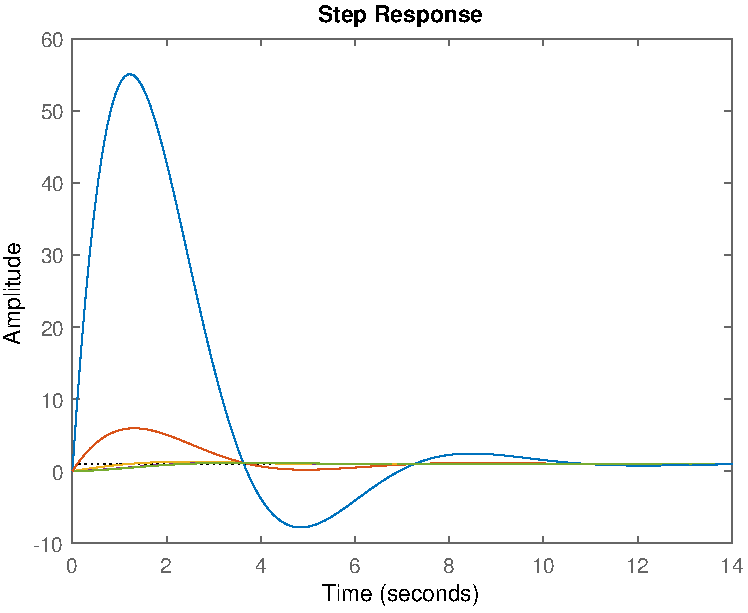
\includegraphics[width=3.5in]{problem2a.pdf}
    \end{center}
\end{figure}
The plot with the highest peak is the transfer function with \(z=0.01\). As the zero
increases in magnitude, the overshoot decreases.

\paragraph{b)}

I ran the following code.
\begin{verbatim}
stepinfo(H1)
stepinfo(H2)
stepinfo(H3)
stepinfo(H4)
stepinfo(H5)
\end{verbatim}
The following table summarizes the percentage overshoot.
\begin{center}
    \begin{tabular}{c|c}
        \(z\) & Overshoot (\%)\\
        \hline
        0.01 & 5407.3\\
        0.1 & 494.331\\
        1 & 29.8352\\
        10 & 16.3862\\
        100 & 16.2988
    \end{tabular}
\end{center}

\paragraph{c)}

I ran the following code.
\begin{verbatim}
option = bodeoptions;
option.PhaseVisible = 'off';
bode(H1, option);
hold on;
bode(H2, option);
bode(H3, option);
bode(H4, option);
bode(H5, option);
hold off;
export_fig problem2c-mag.pdf;

option.PhaseVisible = 'on';
option.MagVisible = 'off';
bode(H1, option);
hold on;
bode(H2, option);
bode(H3, option);
bode(H4, option);
bode(H5, option);
hold off;
export_fig problem2c-phase.pdf;
\end{verbatim}
This generated the following plots.
\begin{figure}[H]
    \begin{center}
        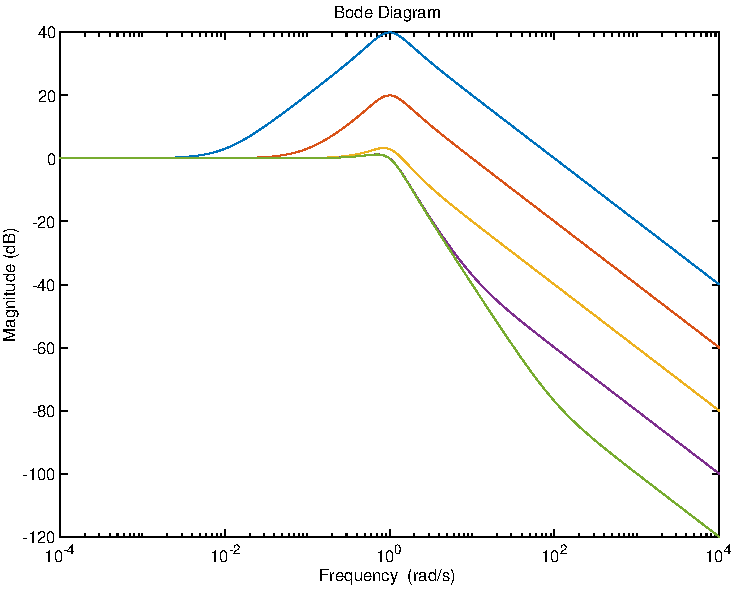
\includegraphics[width=2.5in]{problem2c-mag.pdf}
        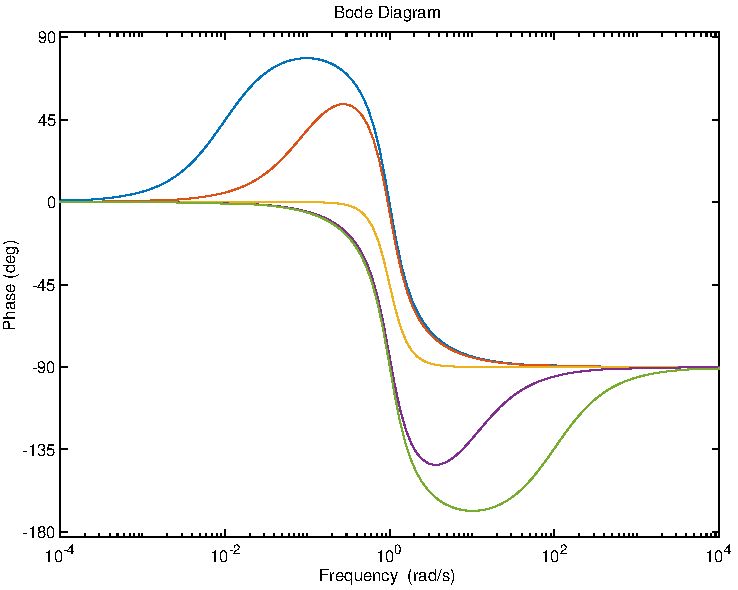
\includegraphics[width=2.5in]{problem2c-phase.pdf}
    \end{center}
\end{figure}

\paragraph{d)}

I ran the following code.
\begin{verbatim}
getPeakGain(H1)
getPeakGain(H2)
getPeakGain(H3)
getPeakGain(H4)
getPeakGain(H5)
\end{verbatim}
The following table summarizes the resonant peaks.
\begin{center}
    \begin{tabular}{c|c}
        \(z\) & Resonant Peak\\
        \hline
        0.01 & 100.0050\\
        0.1 & 10.0499\\
        1 & 1.4676\\
        10 & 1.1495\\
        100 & 1.1547
    \end{tabular}
\end{center}

\paragraph{e)}

As the zeros move further away from the origin, the frequency response has a smaller magnitude and smaller bandwidth.
This is seen in the bode plot because the crossover frequency becomes smaller as the zeros increase in magnitude.
The peak also becomes smaller as the zeros increase in magnitude. In the time response, zeros that are very close
to the origin have large overshoot and cause oscillations. Zeros that are further away have less overshoot and
some do not oscillate at all.

\section*{Problem 3}

\paragraph{a)}

I ran the following code.
\begin{verbatim}
s=tf('s');
H1=1/((s/0.01+1)*(s^2+s+1));
H2=1/((s/0.1+1)*(s^2+s+1));
H3=1/((s/1+1)*(s^2+s+1));
H4=1/((s/10+1)*(s^2+s+1));
H5=1/((s/100+1)*(s^2+s+1));

set(gcf,'color','w');
step(H1);
hold on;
step(H2);
step(H3);
step(H4);
step(H5);
hold off;
export_fig problem3a.pdf;
\end{verbatim}
This output the following plot.
\begin{figure}[H]
    \begin{center}
        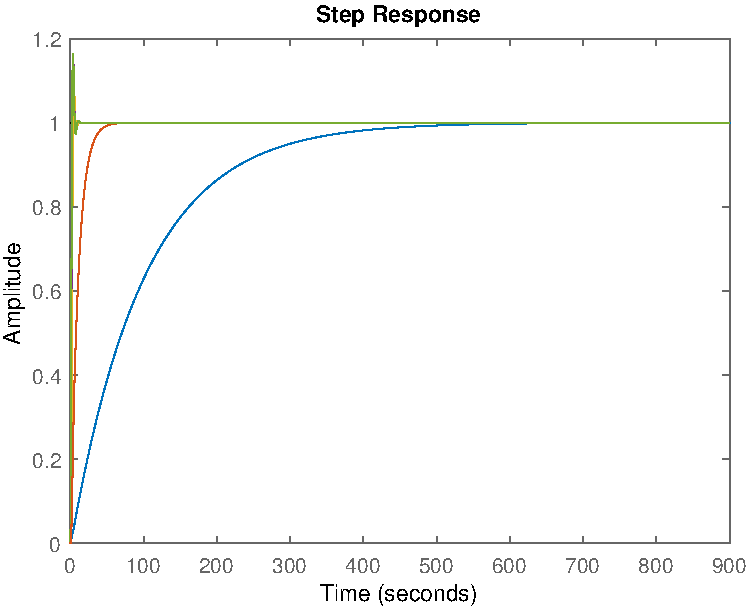
\includegraphics[width=3.5in]{problem3a.pdf}
    \end{center}
\end{figure}
The plot with the longest settling time corresponds to \(p=0.01\).

\paragraph{b)}

I ran the following code.
\begin{verbatim}
stepinfo(H1)
stepinfo(H2)
stepinfo(H3)
stepinfo(H4)
stepinfo(H5)
\end{verbatim}
The following table summarizes the percentage overshoot.
\begin{center}
    \begin{tabular}{c|c}
        \(z\) & Overshoot (\%)\\
        \hline
        0.01 & 0\\
        0.1 & 0\\
        1 & 8.1391\\
        10 & 16.2014\\
        100 & 16.2853
    \end{tabular}
\end{center}

\paragraph{c)}

I ran the following code.
\begin{verbatim}
option = bodeoptions;
option.PhaseVisible = 'off';
bode(H1, option);
hold on;
bode(H2, option);
bode(H3, option);
bode(H4, option);
bode(H5, option);
hold off;
export_fig problem3c-mag.pdf;

option.PhaseVisible = 'on';
option.MagVisible = 'off';
bode(H1, option);
hold on;
bode(H2, option);
bode(H3, option);
bode(H4, option);
bode(H5, option);
hold off;
export_fig problem3c-phase.pdf;
\end{verbatim}
This generated the following plots.
\begin{figure}[H]
    \begin{center}
        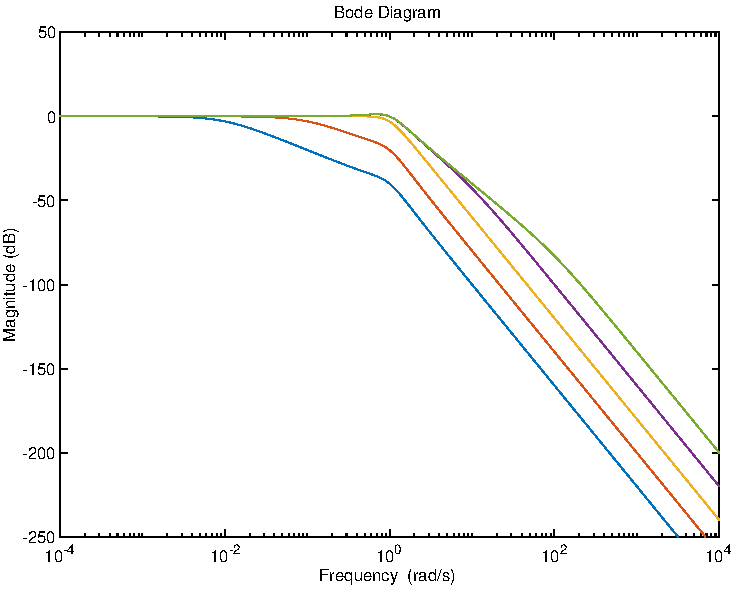
\includegraphics[width=2.5in]{problem3c-mag.pdf}
        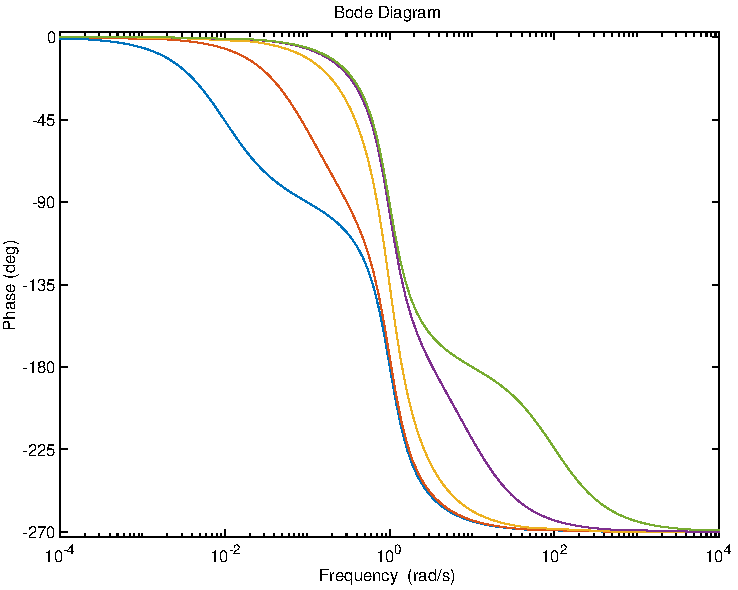
\includegraphics[width=2.5in]{problem3c-phase.pdf}
    \end{center}
\end{figure}

\paragraph{d)}

I ran the following code.
\begin{verbatim}
getPeakGain(H1)
getPeakGain(H2)
getPeakGain(H3)
getPeakGain(H4)
getPeakGain(H5)
\end{verbatim}
The following table summarizes the resonant peaks.
\begin{center}
    \begin{tabular}{c|c}
        \(z\) & Resonant Peak\\
        \hline
        0.01 & 1\\
        0.1 & 1\\
        1 & 1\\
        10 & 1.1518\\
        100 & 1.1547
    \end{tabular}
\end{center}

\paragraph{e)}

As the third pole moves away from the origin, the time response improves and the settling time decreases significantly.
However, this leads to overshoot and less stability. In the frequency response, we can see that there is a higher
bandwidth and greater response magnitude as the pole magnitude increases. So less frequencies are attenuated.

\section*{Problem 4}

\paragraph{a)}

Let the leftmost resistor and capacitor have a combined impedance of \(Z_1\). Let
the remaining resisters and capacitors have a combined impedance of \(Z_2\). Then have the following.
\begin{align*}
    \frac{V_i-V_1}{Z_1}+\frac{V_o-V_1}{Z_2}&=0\\
    Z_2V_i-(Z_1+Z_2)V_1+Z_1V_o&=0\\
    V_1&=\frac{Z_2}{Z_1+Z_2}V_i + \frac{Z_1}{Z_1+Z_2}V_o\\
\end{align*}
Since we assume this is an ideal OpAmp, the voltage that enters the negative terminal is effectively zero.
Thus our transfer function is the following.
\[\frac{V_o}{V_i}=-\frac{Z_2}{Z_1}\]

\paragraph{b)}

\paragraph{c)}

\paragraph{d)}

\section*{Problem 5}

\paragraph{a)}

Experimentally I used MATLAB to obtain the following transfer function.
\[H(s)=\frac{400\left(\left(\frac{s}{10}\right)+1\right)\left(\left(\frac{s}{10000}\right)+1\right)}{(s+1)\left(\left(\frac{s}{100}\right)+1\right)\left(\left(\frac{s}{1000}\right)+1\right)}\]

\paragraph{b)}

The system is type 0, since there are no pure integrators. This is apparent since a pure integrator would cause the bode plot to have a negative slope on the left side, but this
bode plot is flat. The steady state value of the open loop system is \(K_p=400\) from the final value theorem. Then the error constant for the closed loop
system is also \(400\).

\paragraph{c)}

The steady state tracking error for a step input in a unity feedback loop would be \(\frac{1}{1+K_p}=\frac{1}{401}\).

\section*{Problem 6}

\paragraph{a)}

We can calculate \(\zeta\) from the peak gain.
\begin{align*}
    \frac{1}{2\zeta\sqrt{1-\zeta^2}}&=10^{0.6}\\
    \zeta&=0.126613
\end{align*}
We have \(\omega_r=0.9=\omega_n\sqrt{1-2\zeta^2}\). Then we can solve for \(\omega_n\).
\begin{align*}
    \omega_n&=\frac{0.9}{\sqrt{1-2\zeta^2}}\\
    &=0.91478
\end{align*}
Then the best second order approximation for this system is the following.
\[H(s)=\frac{0.83682}{s^2+0.231647s+0.83682}\]

\paragraph{b)}

Using MATLAB I obtained the system bandwidth \(\omega=1.4047\).

\paragraph{c)}

\[e^{-\frac{\pi\zeta}{\sqrt{1-\zeta^2}}}=0.66965\]
The percentage overshoot is approximately 66.965\%.

\end{document}